\documentclass[a4paper, 11pt]{report}
\usepackage[british]{babel}
\usepackage{times}
\usepackage{amsmath}
\usepackage{mathtools}
\usepackage{amsfonts}
\usepackage{verbatim}
\usepackage{natbib}
\usepackage{lmodern}
\usepackage{tikz}
\usepackage{graphicx}
\usepackage[ruled,vlined]{algorithm2e}
\usetikzlibrary{patterns}
\setcitestyle{authoryear,open={[},close={]}}


\numberwithin{equation}{chapter}

\newtheorem{lemma}{Lemma}[chapter]

\DeclareMathOperator*{\argmax}{arg\,max}
\DeclareMathOperator*{\argmin}{arg\,min}

\DeclareMathOperator*{\KL}{{\rm KL}}
\DeclareMathOperator*{\const}{{\rm const}}

\setlength{\parskip}{1em}
\usepackage[a4paper,top=4cm,bottom=4cm,left=3cm,right=3cm,marginparwidth=1.75cm]{geometry}

\title{Averaged Variational Inference for Hierarchical Modelling of Genetic Association}
\author{William van Rooij}
\begin{document}
\SetEndCharOfAlgoLine{}


\begin{titlepage}

\newcommand{\HRule}{\rule{\linewidth}{0.5mm}} % Defines a new command for the horizontal lines, change thickness here

%----------------------------------------------------------------------------------------
%	LOGO SECTION
%----------------------------------------------------------------------------------------
\center

\includegraphics[width=8cm]{images/EPFL_logo.png}\\[1cm] % Include a department/university logo - this will require the graphicx package
 
%----------------------------------------------------------------------------------------


%----------------------------------------------------------------------------------------
%	HEADING SECTIONS
%----------------------------------------------------------------------------------------
\quad\\[1.5cm]
%\textsc{\LARGE MSc Thesis}\\[1.5cm] % Name of your university/college
\textsc{\Large École Polytechnique Fédérale de Lausanne}\\[0.5cm] % Major heading such as course name

%----------------------------------------------------------------------------------------
%	TITLE SECTION
%----------------------------------------------------------------------------------------
\makeatletter
\HRule \\[0.4cm]
{ \huge \bfseries \@title}\\[0.4cm] % Title of your document
\HRule \\[1.5cm]
 
%----------------------------------------------------------------------------------------
%	AUTHOR SECTION
%----------------------------------------------------------------------------------------

\begin{minipage}{0.4\textwidth}
\begin{flushleft} \large
\emph{Author:}\\
\@author % Your name
\end{flushleft}
\end{minipage}
~
\begin{minipage}{0.4\textwidth}
\begin{flushright} \large
\emph{Supervisors:} \\
Dr. Hélène Ruffieux\\
Prof. Anthony Davison 
% Uncomment the following lines if there's a co-supervisor
%\\[1.2em] % Supervisor's Name
%\emph{Co-Supervisor:} \\
%Dr. Adam Smith % second marker's name
\end{flushright}
\end{minipage}\\[3cm]
\makeatother


%----------------------------------------------------------------------------------------
%	DATE SECTION
%----------------------------------------------------------------------------------------

{\large A thesis submitted for the degree of}\\[0.5cm]
{\large \emph{MSc in Applied Mathematics}}\\[0.5cm]
{\large \today}\\[2cm] % Date, change the \today to a set date if you want to be precise

\vfill % Fill the rest of the page with whitespace

\end{titlepage}



\newpage
\begin{abstract}
Expression quantitative trait locus (eQTL) analyses study the effects of genetic variants on the expression of transcripts or genes. The data used generally consist of several hundred thousand genetic variants and thousands of transcript expression outcomes. 

In this work, we suppose that the data follow a hierarchical regression model linking the genetic variants and the outcomes. We are then confronted with a \textit{small n, large p, large q} situation, where $n$ is the number of samples, $p$ is the number of genetic variants, and $q$ is the number of expression levels. In this situation, MCMC algorithms are not suitable for Bayesian inference as their computational cost is too large. 

Here, we present a fast variational algorithm to estimate the associations between genetic variants and traits, based on \citet{eff_inf}. We perform a weighted average of variational estimates obtained from different parameter initialisations and augment our method with simulated annealing.

We evaluate the performance of our proposal by comparing it to existing approaches and assess its accuracy through comparisons with MCMC inference on a small problem.

The code for all our numerical experiments is freely accessible at \\
https://github.com/WilliamVanRooij/MasterProject.
\end{abstract}
\tableofcontents
\newpage
\chapter{Introduction}
\section{Situation}
For the past years, data science has been increasingly present in the world. From financial establishments to road management companies, a lot of industry sectors are integrating data science into their businesses. With improvements in computer performance, we are able to implement faster computation and can work with more complex models. The volume of available, hence analysable, data is also growing, which allows more accurate inference.

Often, when trying to find a model for data, we have many more observations than parameters to fit: a \textit{large n, small p} situation. This is the most common type of statistical analysis. 

Bayesian hierarchical modelling is a valuable tool to identify the dependencies across multiple sources of information, but the number of parameters may be much larger than the number of observations. This is often the case in genomic research, where the situation is called \textit{small n, large p}. Traditional techniques do not apply then, because of both statistical and computational constraints.

In this thesis, we will focus on the \textit{small n, large p} situation in the context of genetic association. We will tackle high-dimensional regression in the Bayesian framework, with its statistical advantages and its computational problem, which often dissuades users from adopting this solution in statistical applications.

\section{Motivation}
Current technology allows us to numerically represent the human genome: a whole new set of data is available to study the influence of the genome on diseases or phenotypes.  Some of these newly-available data measure \textit{genetic variants}, changes at specific locations on  the genome (loci), the different versions of which are called \textit{alleles}. We will focus on the most common category of genetic variants, namely, \textit{single nucleotide polymorphisms} (SNPs), i.e., variations in the nucleotides that are present to some appreciable extent in the population. Some combinations of SNPs are inherited together, which yields block-wise dependence structures.

Figure \ref{fig:corr} shows the correlations between real SNPs, located in region ENm014 on the seventh chromosome, from a Yoruba population \citep[][]{hapmap}. We clearly see a local block structure; outside the blocks, the correlations are not null but very small. A strong block correlation structure means that two SNPs in the same block may be statistically hard to differentiate. The goal is to represent the probabilities of association between a SNP and a trait of interest, while conveying the uncertainty implied by the block correlation in our results.

\begin{figure}[h!]
\centering
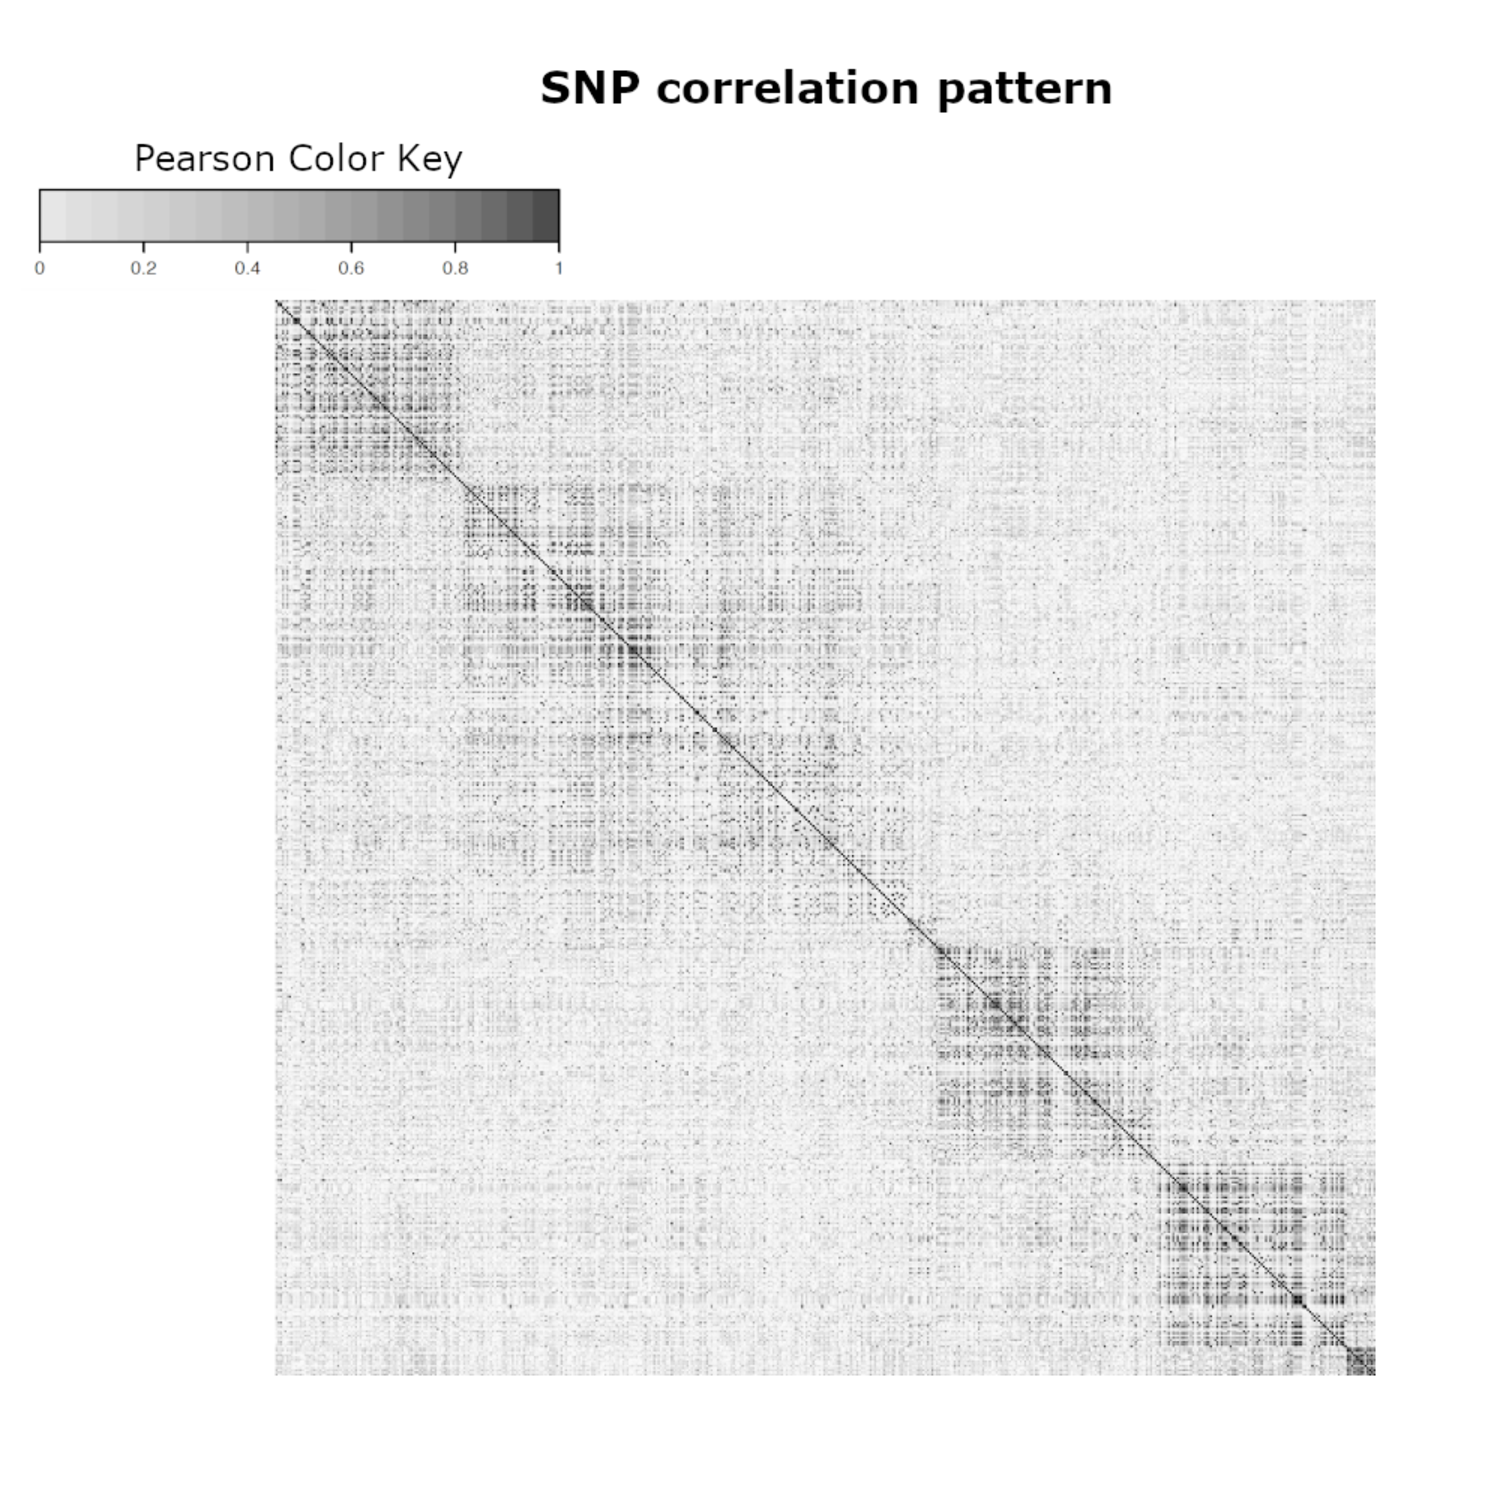
\includegraphics[width=5in]{images/corrRealSNPs.pdf}
\caption{\label{fig:corr} Block correlation structure of SNPs taken from a Yoruba population HapMap, ENm014 region, chromosome $7$ \citep{hapmap}. The darker the dot, the stronger the correlation between the two corresponding SNPs.}
\end{figure}

We focus on \textit{expression quantitative trait locus} (eQTL) analyses, which study the effects of genetic variants, in our case SNPs, on the expression of transcripts or genes. The data used for eQTL studies generally consist of several hundred thousand SNPs and thousands of expression outcomes. It is, in fact, a \textit{small n, large p, large q} situation, where $n$ is the number of samples, $p$ is the number of SNPs, and $q$ is the number of expression outcomes.

Bayesian inference involves many integrals, which usually need to be approximated. Markov Chain Monte Carlo (MCMC) algorithms are a standard technique for the approximation of integrals and can be fast and accurate when working on reasonably small datasets. When the dataset dimensions grow, however, MCMC algorithms tend to become very time-consuming. Indeed, when performing MCMC inference, likelihoods and sometimes gradients typically need to be calculated at each iteration, and the cost of these calculations increases with the number of parameters. Moreover, the higher the dimension, the less accurate the approximations, and more iterations are needed to reach a given precision. For the algorithm to end, all the parameters need to have converged, meaning that they all need to be checked and stored, which is often impossible when their number is very high.

In our \textit{small n, large p, large q} situation, the computational cost of using an MCMC algorithm is huge. The time and memory needed to run the algorithm are unacceptable. We have to use an alternative solution, which we choose to be variational inference \citep{varInf}. 

%==========================================
\newpage
\chapter{Hierarchical sparse regression for multiple responses}
\section{Model}
Let $\boldsymbol{X }= (X_1,\ldots,X_p)$ be a centered design matrix, representing the candidate predictor SNPs, and let $\boldsymbol{y} = (y_1,\ldots,y_q)$ be a centered response matrix, representing the traits. We consider a hierarchical model, where each response $\boldsymbol{y}_t$ is linearly related with the predictors $\boldsymbol{X}$ and has a residual precision $\tau_t$, i.e.,
\begin{equation*}
\label{eq:model}
\boldsymbol{y}_{n\times q} = \boldsymbol{X}_{n \times p}\;\boldsymbol{\beta}_{p \times q}+\boldsymbol{\epsilon}_{n \times q},\quad\boldsymbol{\epsilon}_t \sim \mathcal{N}(0,\tau_t^{-1}I_n),
\end{equation*}
where $\boldsymbol{\beta}$ is the matrix of regression coefficients. The parameters $\tau_t$ and $\sigma^{-2}$ are assigned Gamma priors.

We introduce $\boldsymbol{\gamma}_{p\times q}$, a binary matrix to indicate which pairs of SNPs and traits are associated. The SNP $s$ and trait $t$ are associated if and only if $\gamma_{st} = 1$. To enforce sparsity on $\boldsymbol{\beta}$, we set a ``spike-and-slab'' prior distribution on $\beta_{st}$, i.e.,
\begin{equation*}
\beta_{st} \mid \gamma_{st},\sigma^2, \tau_t \sim \gamma_{st}\;\mathcal{N}(0,\sigma^2\tau_t^{-1})+(1-\gamma_{st})\;\delta_0,
\end{equation*}
where $\delta_0$ is the Dirac distribution.

The prior distribution of $\gamma_{st}$ is
\begin{equation*}
\gamma_{st} \mid \omega_s \sim  \text{Bernoulli}(\omega_s),
\end{equation*}
where the parameter $\omega_s$ controls to the proportion of responses associated with the predictor $\boldsymbol{X}_s$, and follows a Beta distribution,
\begin{equation*}
\omega_s \sim \text{Beta}(a_s, b_s),
\end{equation*}
with parameters $a_s$ and $b_s$ chosen to enforce sparsity. If we assume that $p^* \ll p$, an expected number of predictors involved in the model, we set $a_s$ and $b_s$ such that the prior probability that $\boldsymbol{X}_s$ is associated with at least one response is equal to $p^*/p$. As we fix the mean of the distribution but let the variance be free, there is still one degree of freedom, so multiple choices are possible, e.g.,
\begin{equation*}
a_s = 1,\quad b_s = q(p-p^*)/p^*,
\end{equation*}
 as in \citet{bay_lin}.

Parameters $\sigma$ and $\omega_s$ are shared across all $q$ traits, which enables the borrowing of strength across all traits having predictors in common. 

\section{Parameters of interest for variable selection}

We are interested in estimating the associations between the SNPs and the traits by obtaining summaries of the posterior distribution of $\boldsymbol{\gamma}$ or $\boldsymbol{\beta}$, e.g., for the latter,
\begin{align*}
p(\boldsymbol{\beta}\mid\boldsymbol{y})&=\int\dots\int p(\boldsymbol{\beta},\boldsymbol{\gamma},\boldsymbol{\omega},\boldsymbol{\tau},\sigma^{-2}\mid\boldsymbol{y})\;\mathrm{d}\boldsymbol{\gamma}\;\mathrm{d}\boldsymbol{\omega}\;\mathrm{d}\boldsymbol{\tau}\;\mathrm{d}\sigma^{-2}\\
&=\frac{1}{p(\boldsymbol{y})}\int\dots\int p(\boldsymbol{y},\boldsymbol{\beta},\boldsymbol{\gamma},\boldsymbol{\omega},\boldsymbol{\tau},\sigma^{-2})\;\mathrm{d}\boldsymbol{\gamma}\;\mathrm{d}\boldsymbol{\omega}\;\mathrm{d}\boldsymbol{\tau}\;\mathrm{d}\sigma^{-2},
\end{align*}
with 
\begin{align*}
p(\boldsymbol{y},\boldsymbol{\beta},\boldsymbol{\gamma},\boldsymbol{\omega},\boldsymbol{\tau},\sigma^{-2}) = &\left\lbrace\prod_{t=1}^qp(\boldsymbol{y}_t \mid \boldsymbol{\beta}_t,\tau_t)\right\rbrace\left\lbrace\prod_{t=1}^q\prod_{s=1}^p p(\beta_{st} \mid \gamma_{st},\tau_t,\sigma^{-2})\right\rbrace\\
&\times \left\lbrace \prod_{t=1}^q\prod_{s=1}^p p(\gamma_{st} \mid \omega_s)\right\rbrace\left\lbrace \prod_{s=1}^p p(\omega_s)\right\rbrace\left\lbrace\prod_{t=1}^q p(\tau_t)\right\rbrace p(\sigma^{-2}),
\end{align*}
where, as mentioned earlier,
\begin{align*}
\boldsymbol{y}_t \mid \boldsymbol{\beta}_t,\tau_t \quad &\sim \quad \mathcal{N}_n\left(\boldsymbol{X}\boldsymbol{\beta}_t,\tau_t^{-1}\boldsymbol{I}_n\right),\\
\beta_{st} \mid \gamma_{st},\tau_t,\sigma^{-2} \quad &\sim \quad \gamma_{st}\mathcal{N}\left(0,\sigma^2\tau_t^{-1}\right)+(1-\gamma_{st})\delta_0,\\
\gamma_{st} \mid \omega_s \quad &\sim \quad \mathrm{Bernoulli}(\omega_s),\\
\omega_s \quad &\sim \quad \mathrm{Beta}(a_s,b_s),\\
\tau_t \quad &\sim \quad \mathrm{Gamma}(\eta_t,\kappa_t),\\
\sigma^{-2} \quad &\sim \quad \mathrm{Gamma}(\lambda, \nu),
\end{align*}
for $t=1,\dots,q$, $s=1,\dots p$, and $\delta_0$ is the Dirac distribution.
% =========================================
\newpage
\chapter{Variational Inference}
\section{General principles} \label{sec:gen_princ}
Variational inference simplifies the estimation of the posterior $p(\boldsymbol{\theta}\mid \boldsymbol{y})$ by approximating it with a simpler density $q(\boldsymbol{\theta})$ in an optimisation problem that minimizes a measure of ``closeness''. More precisely, given a family of densities $\mathcal{D}$ over the parameters, we want to find the distribution \mbox{$q \in \mathcal{D}$} that is the closest to $p(\boldsymbol{\theta} \mid \boldsymbol{y})$ in terms of the Kullback--Leibler divergence
\begin{equation*}
\KL(q\parallel p) := \int q(\boldsymbol{\theta})\log \left(\frac{q(\boldsymbol{\theta})}{p(\boldsymbol{\theta} \mid \boldsymbol{y})}\right) \mathrm{d}\boldsymbol{\theta}.
\end{equation*} 
This was introduced in 1951 by \citet{kl51} and is the most common divergence measure used in statistics and machine learning. It is described as a ``directed divergence'' as it is asymmetric, i.e.,
$$
\KL(p\parallel q) \neq \KL(q \parallel p).
$$

Choosing the family $\mathcal{D}$ can be difficult, as we need it to be simple enough to enable tractable inference, but flexible enough for $q$ to accurately represent $p(\boldsymbol{\theta} \mid \boldsymbol{y})$. The approximation will then be
\begin{equation*}
q^*(\boldsymbol{\theta} ) = \argmin_{q(\boldsymbol{\theta}) \in \mathcal{D}} \KL\left[ q(\boldsymbol{\theta}) \parallel p(\boldsymbol{\theta} \mid \boldsymbol{y})\right].
\end{equation*}

As its expression involves the marginal likelihood, directly minimizing the Kullback--Leibler divergence can be complicated, depending on the density $p$ that we want to approximate and the density family $\mathcal{D}$ that we want $q$ to belong to. For this reason, we decompose the Kullback--Leibler divergence as
\begin{align*}
\KL\left[q(\boldsymbol{\theta})||p(\boldsymbol{\theta}\mid \boldsymbol{y})\right] &= \mathbb{E}\left[\log q(\boldsymbol{\theta})\right] - \mathbb{E}\left[\log p(\boldsymbol{\theta}\mid \boldsymbol{y})\right]\\
&= \mathbb{E}\left[\log q(\boldsymbol{\theta})\right] - \mathbb{E}\left[\log p(\boldsymbol{y},\boldsymbol{\theta})\right] + \log p(\boldsymbol{y}),
\end{align*}
and introduce the ``evidence lower bound'' on the marginal log-likelihood:
\begin{equation*}
\mathcal{L}(q) = \mathbb{E}\left[\log p(\boldsymbol{\theta},\boldsymbol{y})\right] - \mathbb{E}\left[\log q(\boldsymbol{\theta})\right] =\int q(\boldsymbol{\theta})\log\frac{p(\boldsymbol{y},\boldsymbol{\theta})}{q(\boldsymbol{\theta})}\mathrm{d}\boldsymbol{\theta},
\end{equation*}
i.e., we obtain
\begin{equation*}
\KL(q\parallel p) = \log(p) - \mathcal{L}(q).
\end{equation*}
This means that the Kullback--Leibler divergence is the difference between the marginal log-likelihood, with no effect on the optimisation, and a function $\mathcal{L}(q)$. Hence, minimizing the Kullback--Leibler divergence is the same as maximizing $\mathcal{L}(q)$. The difference lies in the complexity of the problems: minimizing the Kullback--Leibler divergence is typically intractable, but maximizing $\mathcal{L}(q)$ admits a closed form when the family of densities $\mathcal{D}$ is well chosen. For this reason, variational inference uses $\mathcal{L}(q)$ as its objective function.

Jensen's inequality provides another way to see that $\mathcal{L}(q)$ is a lower bound for the marginal log-likelihood,
\begin{align*}
\log p(\boldsymbol{y}) &= \log \int p(\boldsymbol{y}, \boldsymbol{\theta}) \mathrm{d}\boldsymbol{\theta}\\
&= \log \int \frac{p(\boldsymbol{y}, \boldsymbol{\theta})}{q(\boldsymbol{\theta})}q(\boldsymbol{\theta})\mathrm{d}\boldsymbol{\theta}
\\
&\geq \int q(\boldsymbol{\theta}) \log \left\lbrace \frac{p(\boldsymbol{y}, \boldsymbol{\theta})}{q(\boldsymbol{\theta})} \right\rbrace \mathrm{d}\boldsymbol{\theta}\\
&= \mathcal{L}(q).
\end{align*}
Hence, $\log p(\boldsymbol{y}) \geq \mathcal{L}(q)$.

\section{Mean-field approximation}
The complexity of the optimisation problem is directly bound to the complexity of the family of densities $\mathcal{D}$ to which $q(\boldsymbol{\theta})$ belongs. We introduce the mean-field variational family, where the parameters are mutually independent a posteriori, i.e., let $\left\lbrace \theta_j\right\rbrace_{j=1}^J$ be a partition of $\boldsymbol{\theta}$. Then
\begin{equation*}
q(\boldsymbol{\theta}) = \prod_{j=1}^J q_j(\theta_j).
\end{equation*}
We determine the variational factors $q_j(\theta_j)$ by maximizing $\mathcal{L}(q)$. Hence, the variational family does not directly represent the observed data, the variational inference and the data are linked through the optimisation of the evidence lower bound.

In our case, we assume the posterior independence of most of the parameters,
\begin{equation*}
q(\boldsymbol{\theta}) =\left\lbrace\prod_{s=1}^p \prod_{t=1}^q q(\beta_{st}, \gamma_{st})\right\rbrace \left\lbrace\prod_{s=1}^p  q(\omega_s)\right\rbrace \left\lbrace\prod_{t=1}^q q(\tau_t)\right\rbrace q(\sigma^{-2});
\end{equation*}
we keep $\beta_{st}$ and $\gamma_{st}$ grouped in order to obtain a ``spike-and-slab'' form a posteriori for each of the factors, rather than unimodal distributions, which would ignore the multimodal behaviour induced by the spike-and-slab prior.

\begin{figure}[t]
\centering
\begin{tikzpicture}
\draw[thick, ->] (0,-2) -- (0,2);
\draw[thick, ->] (-2,0) -- (2,0);
\fill[pattern=north west lines,opacity=.6,draw] (0,0) circle (1cm);
\draw[rotate=-45] (0,0) ellipse (0.65cm and 2cm);
\node (p) at (2,1.7) {Real posterior};
\node (q) at (2.7,-0.9) {Mean-field approximation};
\node (x1) at (-0.3,2) {$x_1$};
\node (x2) at (2,-0.3) {$x_2$};
\end{tikzpicture}
\caption{\label{fig:mean_field}Example of the mean-field approximation, for a two-dimensional Gaussian distribution (in clear). The mean-field approximation of the posterior distribution is represented by the barred circle. The mean of the approximation agrees with the real mean, but the covariance does not match the covariance of the real posterior.}
\end{figure}

Using the evidence lower bound and the mean-field approximation, we have transformed our problem into a optimisation problem. We now need a way to solve this problem. In the following section, we describe the coordinate ascent algorithm.
% =========================================
\section{Coordinate ascent}
The coordinate ascent algorithm is typically used to solve the optimisation problem arising in mean-field variational inference. It iterates on the variational parameters of the mean-field approximation, optimising them one at the time, and yields a local optimum for the evidence lower bound. The algorithm is based on the following result:
\begin{lemma}

If we fix $q_l(\theta_l)$, $l\neq j$, then the optimal $q^*_j(\theta_j)$ satisfies
\begin{equation*}
q^*_j(\theta_j) \propto \exp\left\lbrace\mathbb{E}_{-j}\left[\log p(\theta_j \mid \boldsymbol{\theta}_{-j}, \boldsymbol{y})\right]\right\rbrace,
\end{equation*}
where $\mathbb{E}_{-j}$ denotes the expectation with respect to all $\theta_l$, $l \neq j$.
\end{lemma}

Based on this result, the algorithm updates one parameter $\theta_j$ at a time while the others stay fixed. The algorithm stops when $\mathcal{L}(q)$ increases by less than a pre-determined tolerance $\varepsilon$.

\begin{algorithm}
\SetKwData{ELBO}{$\mathcal{L}(q)$}\SetKwData{OLDELBO}{$\mathcal{L}^{\text{old}}(q)$}
\SetKwFunction{Union}{Union}\SetKwFunction{FindCompress}{FindCompress}
\SetKwInOut{Input}{input}\SetKwInOut{Output}{output}\SetKwInOut{Init}{initialize}
\SetKw{Set}{set}
\Input{$p(\boldsymbol{y},\boldsymbol{\theta})$, dataset $y$, tolerance $\varepsilon$}
\BlankLine
\Output{$q(\boldsymbol{\theta}) = \prod_{j=1}^J q_j(\theta_j)$}
\BlankLine
\Init{the parameters of each $q(\theta_j)$}
\BlankLine
\Repeat{$|$\OLDELBO$-\mathcal{L}(q)| < \varepsilon $}{
\For{$j\in \left\lbrace 1, \ldots, J \right\rbrace $}{
\Set{$q_j(\theta_j) \propto \exp\left\lbrace\mathbb{E}_{-j}\left[\log p(\theta_j \mid \boldsymbol{\theta}_{-j}, \boldsymbol{y})\right]\right\rbrace$}}
\BlankLine
\OLDELBO$\leftarrow$\ELBO\\
\ELBO$\leftarrow\mathbb{E}\left[\log p(\boldsymbol{\theta}, \boldsymbol{y})\right]-\mathbb{E}\left[\log q(\boldsymbol{\theta})\right]$
\BlankLine
}
\Return{$q(\boldsymbol{\theta})$}
\caption{\label{alg:CAVI}Coordinate ascent variational inference}
\end{algorithm}
At every iteration, $\mathcal{L}(q)$ is guaranteed to increase. The local optimum thus obtained may depend on the initialization of the $q_j(\theta_j)$, $j=1,\ldots,J$; different initializations could yield different optima that correspond to different models.

For our model, the posterior distributions of our model parameters are:
\begin{align*}
\beta_{st} \mid \gamma_{st} = 1, \boldsymbol{y} &\sim \mathcal{N}\left(\mu_{\beta, st},\sigma^2_{\beta, st}\right),\\
\beta_{st} \mid \gamma_{st} = 0, \boldsymbol{y} &\sim \delta_0,\\
\gamma_{st} \mid \boldsymbol{y} &\sim \text{Bernoulli}(\gamma_{st}^{(1)}),\\
\omega_s\mid\boldsymbol{y} &\sim \text{Beta}(a_s^*,b_s^*),\\
\tau_t\mid \boldsymbol{y} &\sim \text{Gamma}(\eta^*_t, \kappa^*_t),\\
\sigma^{-2} \mid \boldsymbol{y} &\sim \text{Gamma}(\lambda^*, \nu^*),
\end{align*}
for $s=1,\dots,p$, $t=1,\dots,q$, where $\mu_{\beta,st}$, $\sigma^2_{\beta,st}$, $\gamma_{st}^{(1)}$, $a_s^*$, $b_s^*$, $\eta_t^*$, $\kappa_t^*$, $\lambda^*$, and $\nu^*$ are the ``variational'' parameters obtained after convergence of Algorithm \ref{alg:CAVI}. Their complete expression is given in Appendix B of \citet{helen}.

\newpage
\chapter{Multimodality}
\section{Problem statement} \label{sec:pro_stat}
When applied to highly correlated data, variational inference underestimates posterior variances, as explained in \citet{varInf}. Suppose that $p(\boldsymbol{\theta} \mid \boldsymbol{y})$ is the posterior distribution of $\boldsymbol{\theta} = (\theta_1,\theta_2)$ and that we use the mean-field approximation $$
q(\boldsymbol{\theta}) = q(\theta_1)q(\theta_2),
$$
as we can see in Figure \ref{fig:mean_field}, the covariance structure is altered, $\theta_1$ and $\theta_2$ are independent a posteriori, and the marginal variances are smaller than those of $p(\boldsymbol{\theta} \mid \boldsymbol{y})$. This also results from the optimisation of the reverse Kullback--Leibler divergence
$$
\KL (q\parallel p) = - \int q(\boldsymbol{\theta})\log\frac{p(\boldsymbol(\theta\mid\boldsymbol{y})}{q(\boldsymbol{\theta})}\mathrm{d}\boldsymbol{\theta},
$$
which penalizes putting mass in $q(\cdot)$ where $p(\cdot)$ has little mass.

The lower bound $\mathcal{L}(q)$ tends to be highly multimodal, so the ascent algorithm (Algorithm~\ref{alg:CAVI}) risks getting stuck in local modes. The posterior variance underestimation reinforces this risk, putting a lot of mass on one single hypothesis.

To handle this multimodality better, we will explore two routes to enhance variational inference, without changing the model. The first is to introduce a simulated annealing procedure to explore more modes; this was proposed by \citet{glob_loc}. The second is to average over multiple parameter initialisations with weights equal to the posterior model probability corresponding to the obtained mode. We describe these two options in Sections \ref{sec:ann} and \ref{sec:var_inf}.
\section{Annealed variational inference} \label{sec:ann}
Simulated annealing aims at improving the exploration of multimodal parameter spaces, using heated distributions to sweep the local modes away and ease the progression to the global mode. We next describe how it can be coupled with variational inference.

We start with the same strategy as in Section \ref{sec:gen_princ}, i.e., minimising the reverse Kullback--Leibler divergence,
\begin{equation*}
\KL(q \parallel q) = -\int q(\boldsymbol{\theta}) \log\left\lbrace\frac{p(\boldsymbol{\theta}\mid\boldsymbol{y})}{q(\boldsymbol{\theta})}\right\rbrace \mathrm{d}\boldsymbol{\theta},
\end{equation*}
and use the lower bound evidence as objective function,
\begin{equation*}
\mathcal{L}(q) = \mathbb{E}_q\left[ \log p(\boldsymbol{y}, \boldsymbol{\theta})\right] - \mathbb{E}_q\left[\log q(\boldsymbol{\theta})\right].
\end{equation*}
The objective function is composed of the expected log joint distribution, which implies that the approximation will put more mass where the variables best explain the data, and the entropy, which encourages the ``dispersion'' of the approximation. 

The idea of simulated annealing is to introduce a temperature $T$ to obtain a series of heated distributions,
\begin{equation*}
p_T(\boldsymbol{y},\boldsymbol{\theta}) \propto p(\boldsymbol{y},\boldsymbol{\theta})^{1/T},
\end{equation*}
and control the ``frequency'' of the modes. The temperature starts high, smoothing the density of interest, and gets lower along the process until the original density is reached. The high temperatures facilitate the search for the global optimum. The temperature multiplies the entropy term, allowing for more disperse approximations
\begin{equation}
\mathcal{L}_T(q_T) = \int q_T(\boldsymbol{\theta}) \log p(\boldsymbol{y},\boldsymbol{\theta})\mathrm{d}\boldsymbol{\theta} - T \int q_T(\boldsymbol{\theta}) \log q_T(\boldsymbol{\theta}) \mathrm{d}\boldsymbol{\theta},\quad T\geq 1,
\label{eq:ann_elbo}
\end{equation}
where $q_T$ is the heated variational distribution. Hence, annealed variational inference applies a penalty on the log joint distribution when the temperature $T > 1$, and relaxes the penalty as $T$ goes down until $T = 1$, where the penalty becomes null.

To obtain the annealed variational factors, $q_T(\theta_j)$, we write (\ref{eq:ann_elbo}) with respect to $\theta_j$ as
\begin{align*}
\mathcal{L}_T(q) &= \mathbb{E}_j\left[\mathbb{E}_{-j}\left\lbrace \log p(\boldsymbol{y},\boldsymbol{\theta})\right\rbrace - T \log q_T(\theta_j)\right]+ \const\\
&= T\mathbb{E}_j\left[\log\left\lbrace\frac{p_{T, -j}(\boldsymbol{y}, \theta_j)}{q_T(\theta_j)}\right\rbrace\right] + \const,	
\end{align*}
where $p_{T, -j}(\boldsymbol{y},\theta_j) \propto \exp\left\lbrace T^{-1}\mathbb{E}_{-j}\left[\log p(\boldsymbol{y},\boldsymbol{\theta})\right]\right\rbrace$, $\mathbb{E}_j$ is the expected value with respect to $q_T(\theta_j)$, $\mathbb{E}_{-j}$ is the expected value with respect to every $ q_T(\theta_k)$ where $k \neq j$, and $\const$ is independent of $\theta_j$. The objective function for $\mathcal{L}_T(q)$ is maximal when $q_T(\theta_j) = p_{T,-j}(\boldsymbol{y},\theta_j)$, i.e., when
\begin{equation*}
\log q_T(\theta_j) = T^{-1} \mathbb{E}_{-j}\left[\log p(\boldsymbol{y}, \boldsymbol{\theta})\right] + \const\text{,}\quad j=1,\dots,J.
\end{equation*}

Different choices are possible for the temperature schedule \citep{helen}, including geometric spacing,
\begin{equation*}
T_l = (1 + \Delta)^{l-1},\quad \Delta = T_L^{1/(L-1)}-1,
\end{equation*}
harmonic spacing,
\begin{equation*}
T_l = 1 + \Delta(l-1), \quad \Delta =\frac{T_L-1}{L-1},
\end{equation*}
and linear spacing,
\begin{equation*}
T_l^{-1} = T_L^{-1} + \Delta (L-l), \quad \Delta = \frac{1-T_L^{-1}}{L-1},
\end{equation*}
where $l = 1,\dots,L$ and $T_L$ is the hottest temperature. $T_l$ is the temperature used at step $l$ and $L$ is the number of steps used to lower the temperature to the initial temperature $T = 1$. The original variational algorithm is then run until convergence.

The choice of temperature schedule is free. In our simulations, in Chapter \ref{chap:sim}, we focus on geometric spacing. The number of steps $L$ usually varies between $10$ and $100$, we use $10$ steps.
\section{Averaged variational inference} \label{sec:var_inf}
Bayesian model averaging is a strategy to account for multiple competing models in an inference problem. It consists of weighting the different models in a weighted average, accounting for the likelihood that the data corresponds to each model. The more the model corresponds to the observed data, the more it will stand out in the result.

Assume that the data $\boldsymbol{y}$ may have been obtained from one of multiple models $M_k$, $k= 1,\ldots,K$, and $\Delta$ is the quantity of interest. The posterior density
\begin{equation}
p(\Delta \mid \boldsymbol{y}) = \sum_{k=1}^K p(\Delta \mid M_k,\boldsymbol{y}) \; p(M_k \mid \boldsymbol{y})
\label{eq:post_dist}
\end{equation}
corresponds to a weighted average of the posterior densities under each of the considered models with weights corresponding to the posterior model probabilities. Instead of $p(\Delta \mid \boldsymbol{y})$ in (\ref{eq:post_dist}), we might be interested in summaries like the posterior mean
\begin{equation*}
\mathbb{E}\left[\Delta \mid \boldsymbol{y}\right] = \sum_{k=1}^K\mathbb{E}\left[\Delta \mid M_k, \boldsymbol{y}\right]\;p(M_k \mid \boldsymbol{y}).
\end{equation*}

The posterior probability for model $M_k$ is
\begin{equation}
p(M_k \mid \boldsymbol{y}) = \frac{p(\boldsymbol{y} \mid M_k)\; p(M_k)}{\sum_{j=1}^K p(\boldsymbol{y} \mid M_j)\; p(M_j)},
\label{eq:post_prob}
\end{equation}
where $p(\boldsymbol{y} \mid M_k)$ is the likelihood under model $M_k$, and $p(M_k)$ is the prior probability of model $M_k$. This may, for example, be chosen based on the model complexity, to favour simpler models, or, if we consider the models to be a priori equiprobable, it is set to $p(M_k) = 1/K$, $k = 1,\ldots,K$.  

In Section \ref{sec:gen_princ}, we saw that the evidence lower bound and the Kullback--Leibler divergence are related, 
\begin{equation*}
\KL(q\parallel p) = \log p (\boldsymbol{y}) - \mathcal{L}(q),
\end{equation*}
and that minimizing the Kullback--Leibler divergence is equivalent to maximizing the evidence lower bound. Hence, if we assume that $\mathcal{L}(q)$ is a tight lower bound on the marginal log likelihood, we can use it as an approximation for $\log p(\boldsymbol{y}\mid M_k)$ in (\ref{eq:post_prob}).

We propose to address the concerns described in Section \ref{sec:gen_princ} by performing a form of averaging of variational inference summaries. Namely, say that our quantity of interest is $\gamma_{st}$, to assess the association between SNP $s$ and trait $t$. Using Algorithm \ref{alg:CAVI}, we initialise the distributions $q_j(\theta_j)$ with different starting points, and consider the optima yielded by the algorithm. If we consider that each optimum yields a model representing the data, we can apply an averaging procedure to combine them all using the method described above. We approximate $\log p(\boldsymbol{y})$ by $\mathcal{L}(q)$ in (\ref{eq:post_prob}), and obtain an approximation for $\mathbb{E}\left[\gamma_{st}\mid \boldsymbol{y}\right]$ considering all the models obtained through the algorithm.

To cope with the high multimodality induced by strongly correlated structures and represent the uncertainty of the modes, we use simulated annealing combined with our weighted averaging procedure and retrieve a combination of different models yielded from different initialisations. We hope that the uncertainty in the selected variables will be conveyed in the resulting approximations for $\mathbb{E}\left[\gamma_{st}\mid \boldsymbol{y}\right]$.

% =========================================
\newpage
\chapter{Simulations} \label{chap:sim}
\section{Preliminary illustration}
In this chapter, we assess the performance of our averaged variational method on simulations. We use the \texttt{R}-package \texttt{locus} \citep{r_locus} and call the variational algorithm multiple times before combining all the results in a weighted average. As explained in Section \ref{sec:var_inf}, we initialise the parameters differently for each call, in order to obtain possibly different optima. Then we use the evidence lower bound of the different calls as weights to combine the posterior summaries of each initialisation. 

For most simulations presented in this chapter, we simulate data with very strong correlation patterns to evaluate the benefit of our method in the extreme multimodality scenarios it is designed for.

We use the \texttt{echoseq R}-package \citep{r_echoseq} to generate blocks of strongly autocorrelated SNPs and traits, as well as associations between them. The SNPs are coded as discrete variables describing their state and we create dependence between them using realisations of multivariate normal variables followed by a quantile thresholding rule.

For our first illustration, we generate $300$ observations of $500$ SNPs, by blocks of $10$ SNPs, with latent variable block autocorrelations between $0.98$ and $0.99$. For simplicity, we simulate just one trait. We select five SNPs to be associated with the trait and, for better visualisation, all five SNPs are among the $50$ first SNPs.


\begin{figure}[h]
\centering
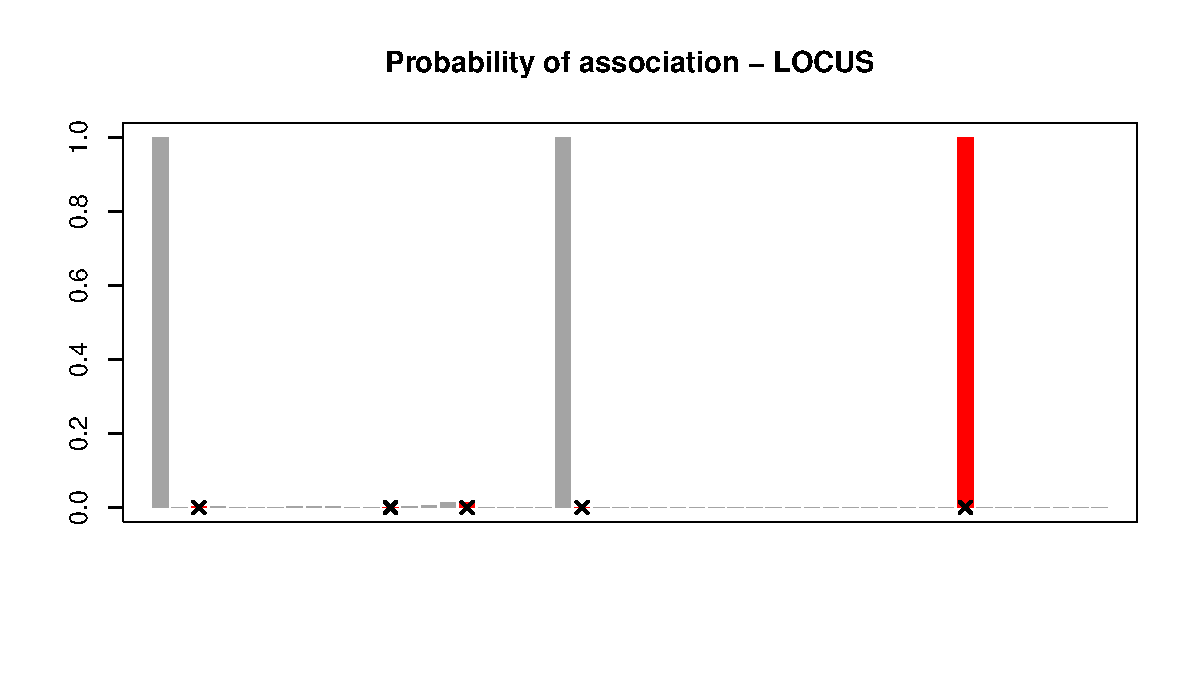
\includegraphics[width=2.9in, bb= 0 0 8in 4in]{images/proba_single.pdf}
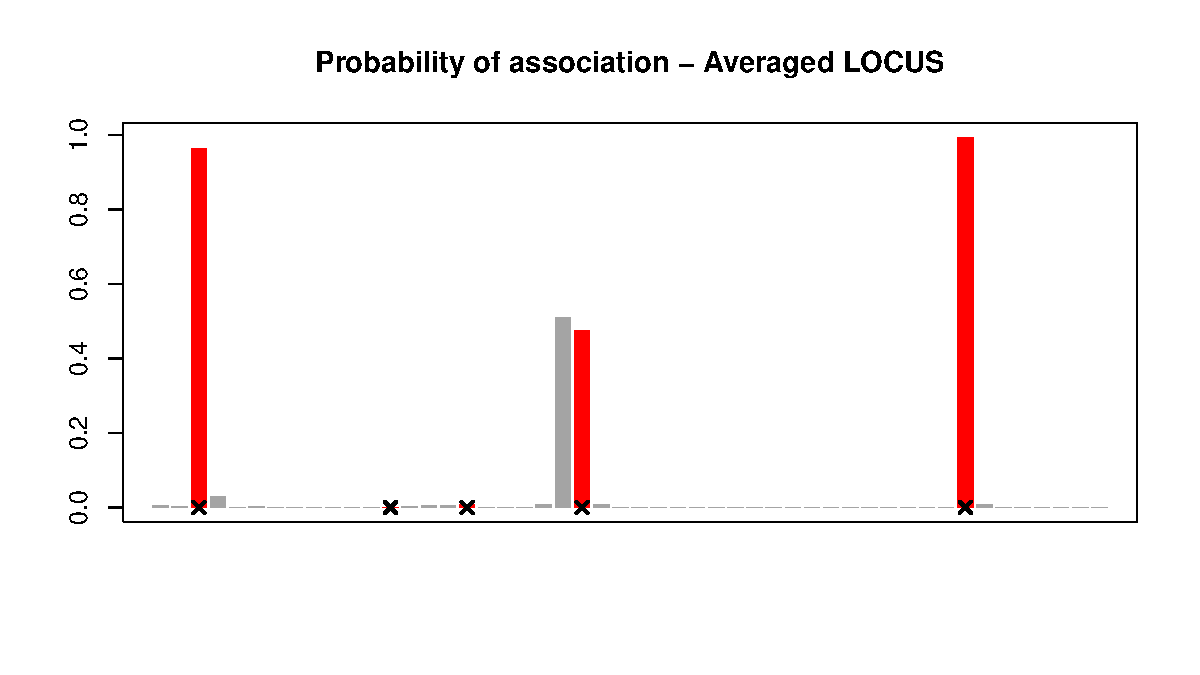
\includegraphics[width=2.9in, bb= 0 0 8in 4in]{images/proba_averaged.pdf}
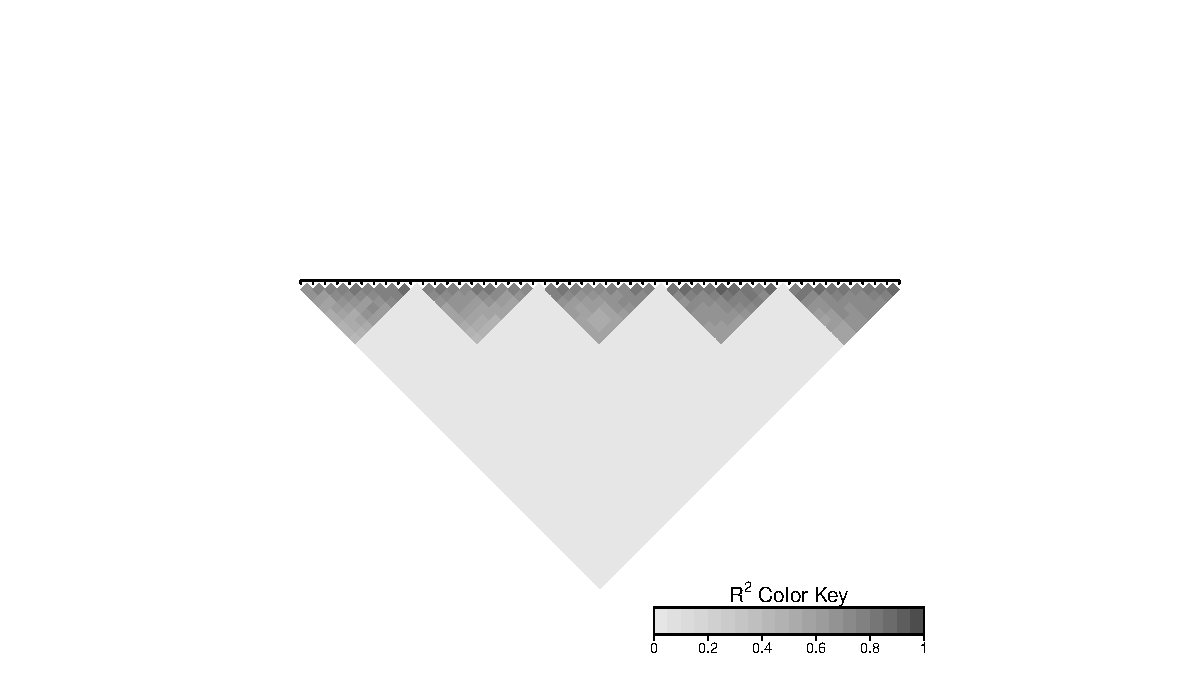
\includegraphics[width=2.9in, bb= 1.32in 0 6.4in 2in]{images/LD_plot.pdf}
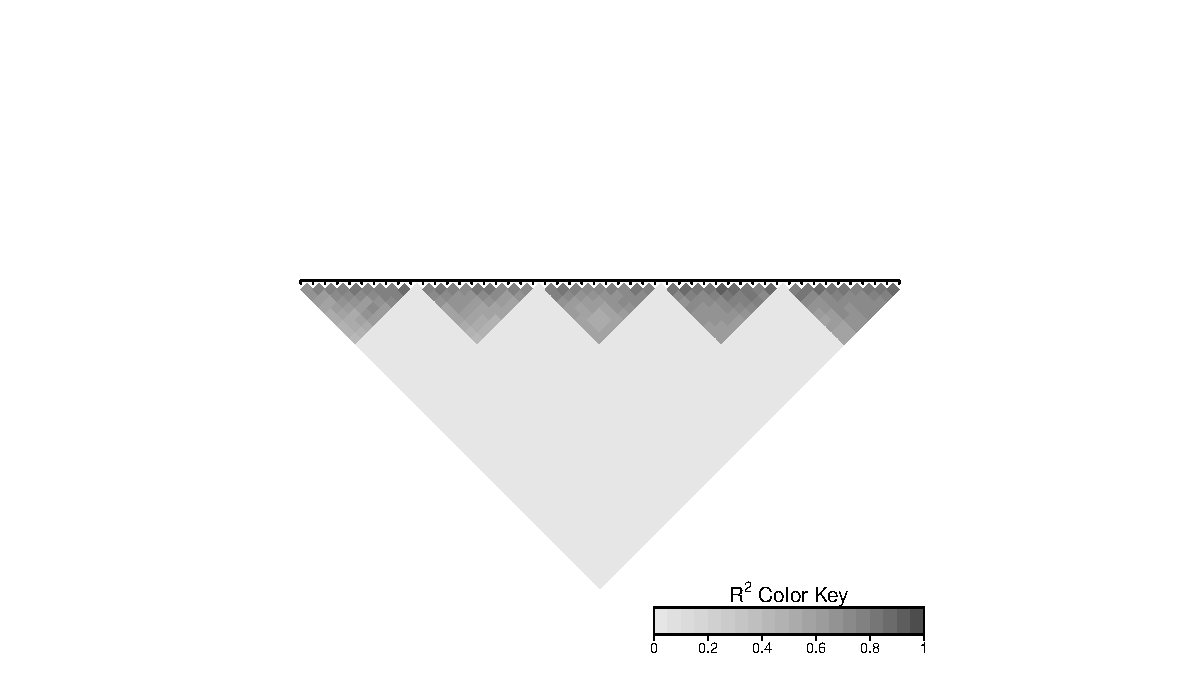
\includegraphics[width=2.9in, bb= 1.32in 0 6.4in 2in]{images/LD_plot.pdf}
\caption{\label{fig:simple_locus}Probabilities of association of the $50$ first SNPs with a single trait estimated using the original LOCUS method (left) and using our ``averaged LOCUS'' proposal (right), which implements the weighted average described in Section \ref{sec:var_inf}. In red are the five SNPs simulated as associated with the response, they are also marked with a black cross. Underneath are the extreme correlation patterns of the SNPs; they are the same for the two sides, as the SNPs used are the same.}
\end{figure}

Figure \ref{fig:simple_locus} shows the probabilities of association of the first $50$ SNPs, out of $500$ simulated. The LOCUS method is equivalent to choosing a single model $M$ and calculating
\begin{equation*}
\mathbb{E}\left[\gamma_{st}\mid\boldsymbol{y}\right] = \mathbb{E}\left[\gamma_{st}\mid M,\boldsymbol{y}\right]\;p\left(M\mid\boldsymbol{y}\right).
\end{equation*}

Our ``averaged LOCUS'' method uses a weighted average over $100$ different initialisations yielding $100$ models $ M_1,\ldots,M_{100}$:
\begin{equation*}
\mathbb{E}\left[\gamma_{st}\mid\boldsymbol{y}\right] = \sum_{k=1}^{100}\mathbb{E}\left[\gamma_{st}\mid M_k\right]\;p\left(M_k\mid\boldsymbol{y}\right).
\end{equation*}

With the original LOCUS method, the algorithm wrongly selects two SNPs and misses four SNPs simulated as associated with the response. This can be explained by the strong correlations in the block structure creating a highly multimodal posterior and misleading the algorithm.

Our averaged variational inference algorithm (averaged LOCUS) does better; it identifies three of the five relevant SNPs. It also better conveys the block correlation structure in the probabilities of association as four SNPs of the middle block all have small but non null probabilities of association with the trait. 

The second correlation block should contain two associated SNPs, and both of the methods seem to have failed to identify them as such. The two SNPs are highly correlated and their effect sizes are $\beta_{13} = 0.63$ and $\beta_{17} = -0.79$. The response $\boldsymbol{y}$ is related to the SNPs $\boldsymbol{X}$ with the model $\boldsymbol{y} \sim \boldsymbol{X} \boldsymbol{\beta} + \boldsymbol{\varepsilon}$, with $\boldsymbol{\varepsilon}$ the error. As the two active SNPs are strongly correlated and have opposite effect sizes, they ``cancel'' each other, making it seem like they had small effect sizes.
 
% This could be a scaling problem. As the averaged LOCUS yields two probabilities of association almost equal to one, the smaller probabilities of association seem negligible.
%
%Figure \ref{fig:probablock} shows the probabilities of association of the second block of SNPs. The probabilities of association are not all null. One of the associated SNPs has a higher probability of being associated than the others. The uncertainty resulting from the high multimodality of the problem is represented here by the probabilities of association of the SNPs between the two associated SNPs that are all above zero. The algorithm couldn't determine which SNP was associated, the correlation between them being too strong.
%
%\begin{figure}[h!]
%\centering
%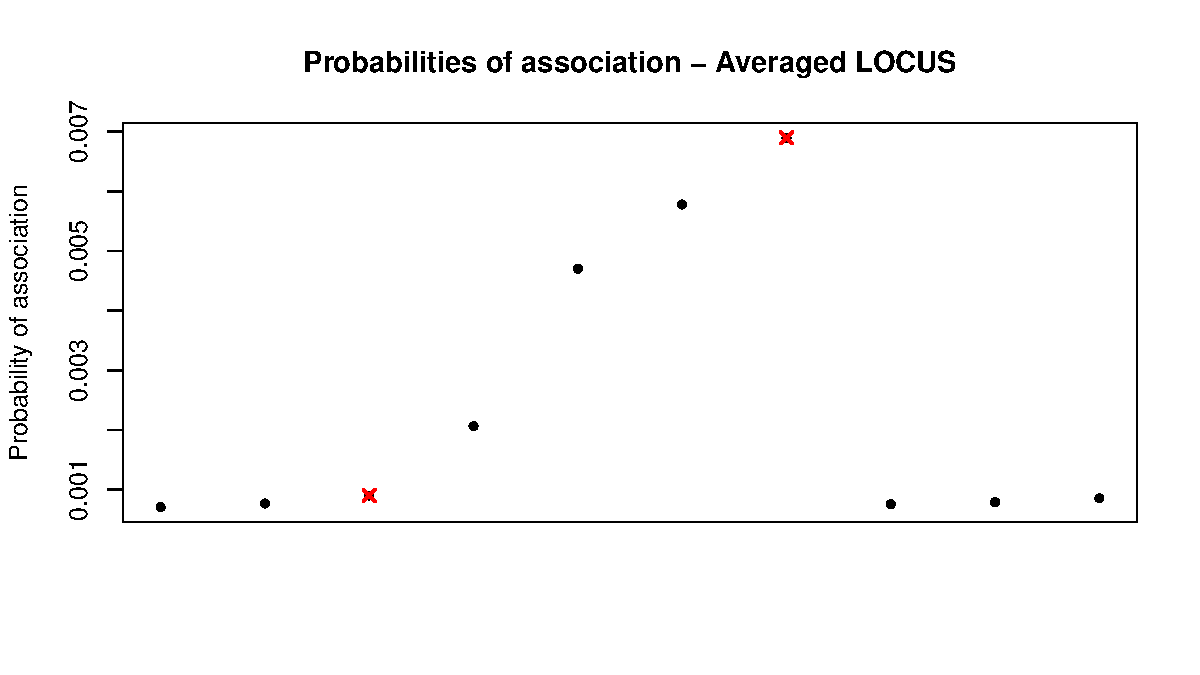
\includegraphics[width=5in, bb=0 0 8in 4.5in]{images/proba_block.pdf}
%\caption{\label{fig:probablock}Probabilities of association for the second block of SNPs, yielded by the averaged LOCUS method. The red crosses indicate the associated SNPs.}
%\end{figure}

Moreover, as we will see in Section \ref{sec:comparison}, when the correlations are too strong and the effect sizes are too small, our method can miss an associated SNP and compensate by adding more weight to the other SNPs. The correlation in our situation is extremely high, but if we reduce it, the algorithm finds all the associated SNPs.

\begin{figure}[h]
\centering
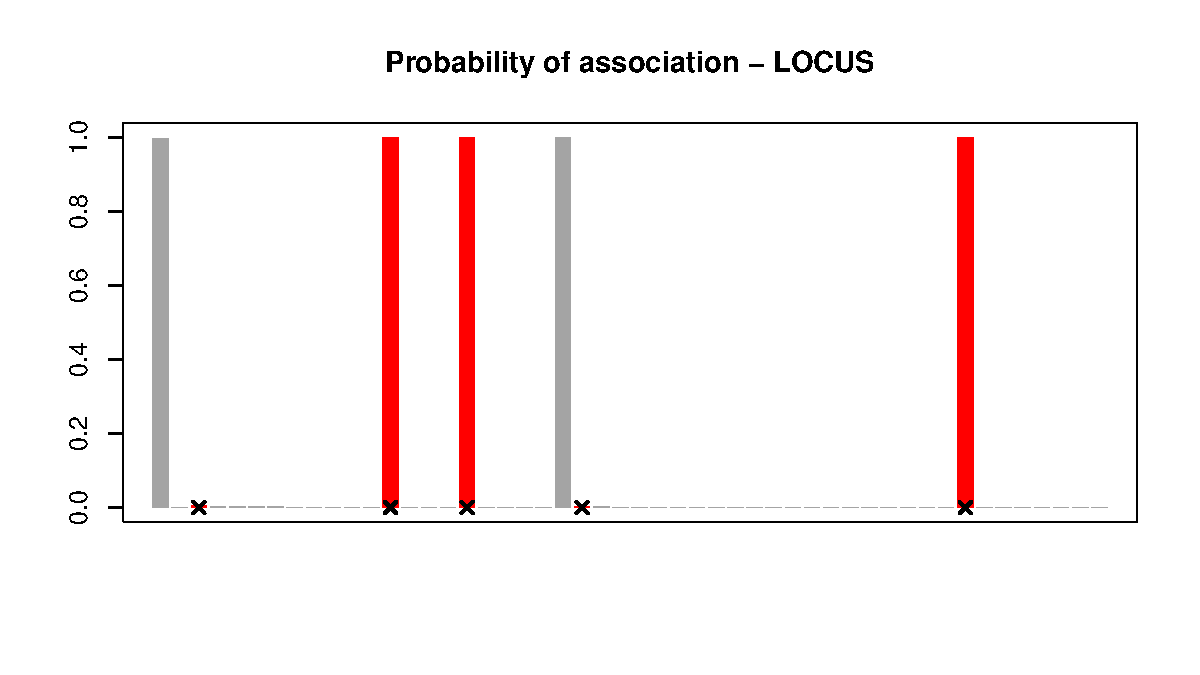
\includegraphics[width=2.9in, bb= 0 0 8in 4in]{images/proba_weak.pdf}
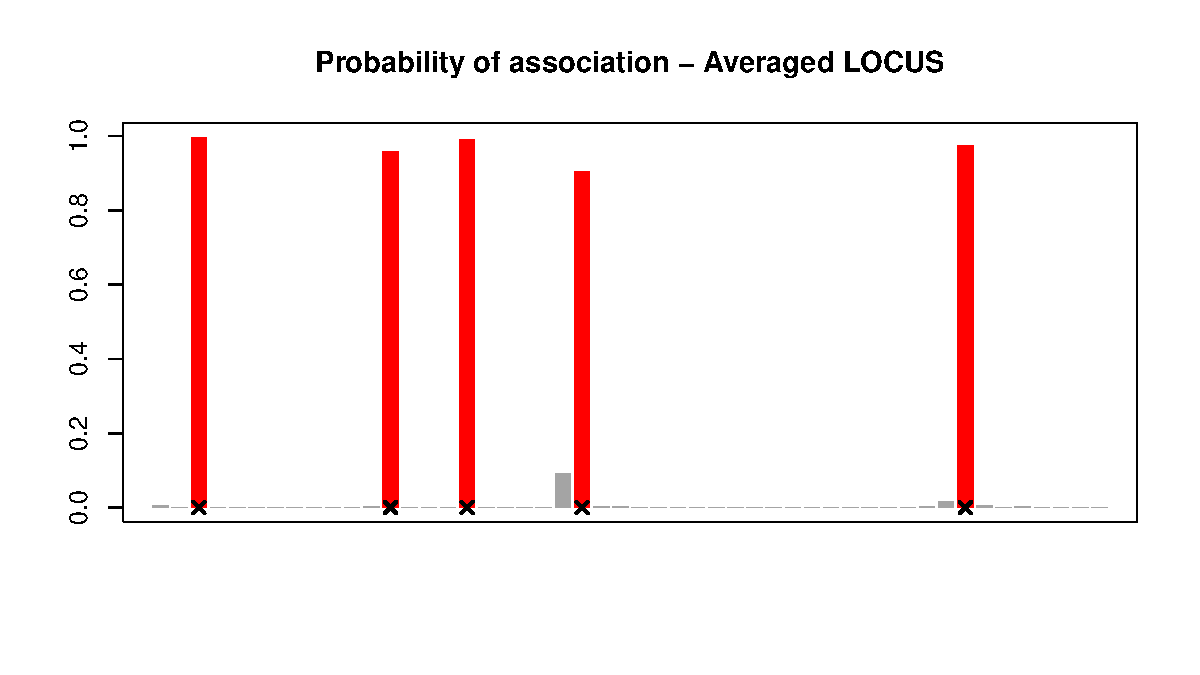
\includegraphics[width=2.9in, bb= 0 0 8in 4in]{images/proba_weak_m.pdf}
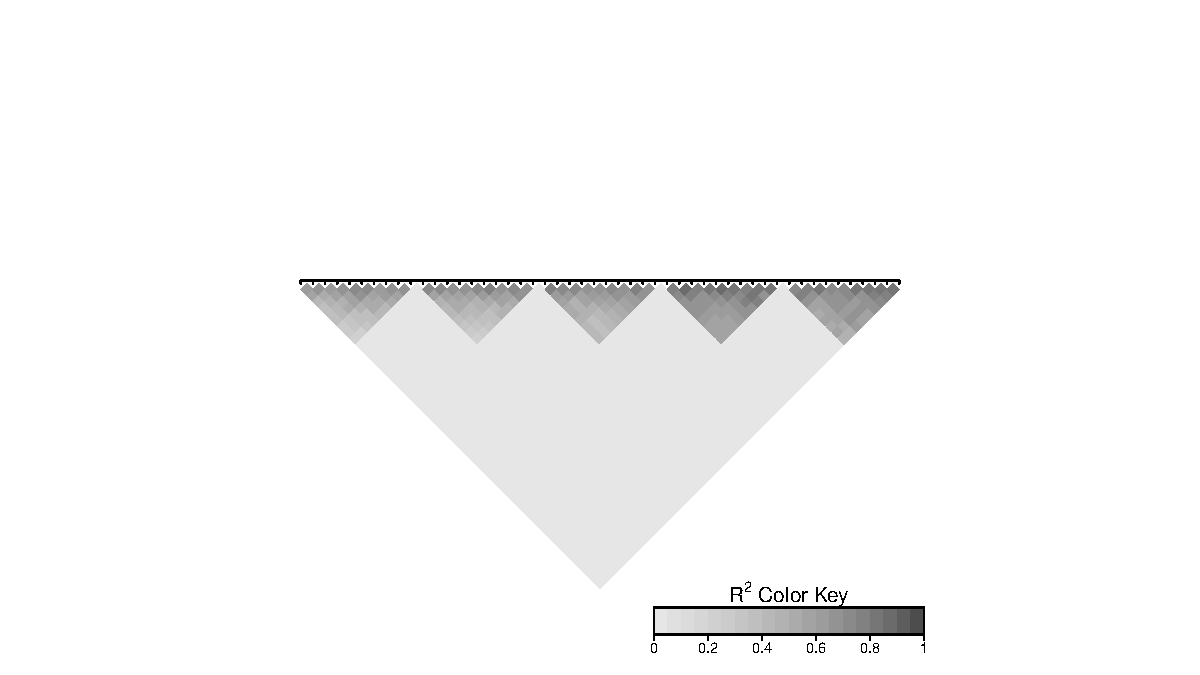
\includegraphics[width=2.9in, bb= 1.32in 0 6.4in 2in]{images/LD_weak.pdf}
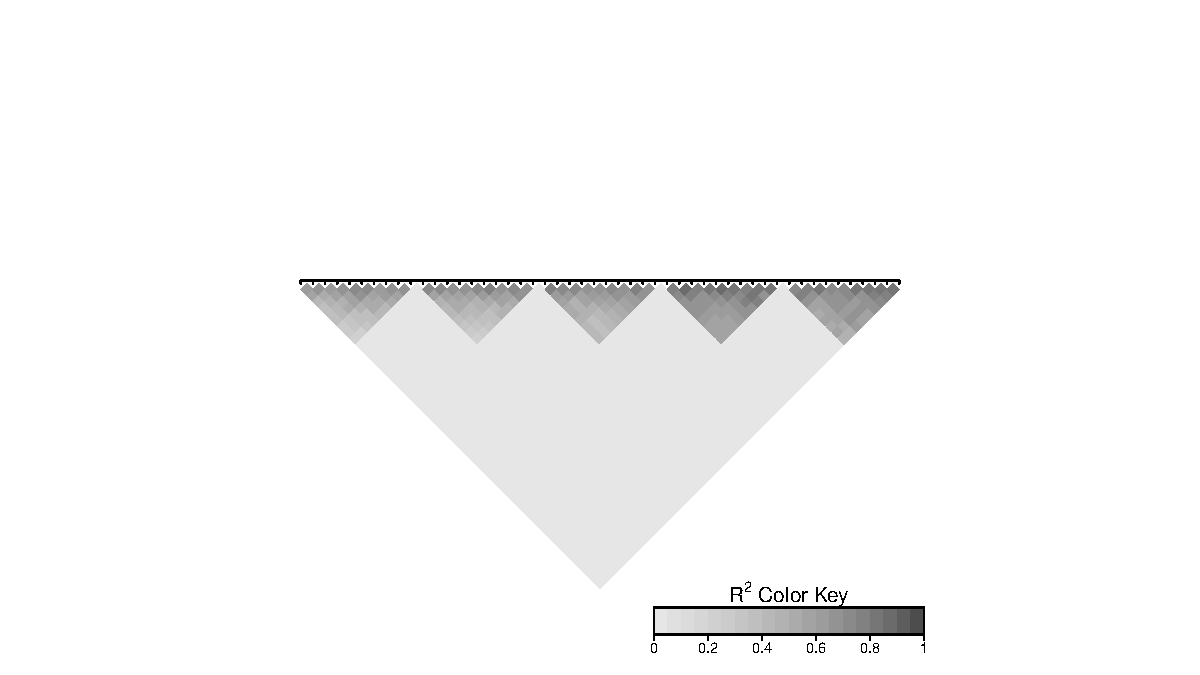
\includegraphics[width=2.9in, bb= 1.32in 0 6.4in 2in]{images/LD_weak.pdf}
\caption{\label{fig:weaker_locus}Probabilities of association of the $50$ first SNPs with a single trait estimated using the original LOCUS method (left) and using our ``averaged LOCUS'' proposal (right), which implements the weighted average described in Section \ref{sec:var_inf}. In red are the five SNPs simulated as associated with the response, they are also marked with a black cross. Underneath are the correlation patterns of the SNPs, they are autocorrelated with an autocorrelation between $0.95$ and $0.99$, which is weaker than for Figure \ref{fig:simple_locus}; they are the same for the two sides, as the SNPs used are the same.}
\end{figure}

Figure \ref{fig:weaker_locus} shows the probabilities of association of the first $50$ SNPs, out of $500$ simulated. The SNPs have weaker correlations as for Figure \ref{fig:simple_locus}, but the same SNPs are associated with the trait. The other settings are the same as for Figure \ref{fig:simple_locus}.

With weaker correlations, it is easier for LOCUS to find associated SNPs, it selects three truly associated SNPs, but the correlations are still too strong and mislead LOCUS into wrongly selecting two SNPs. Averaged LOCUS, however, finds the five correct associated SNPs, and we can still read the uncertainty around the middle correlation block, where a non-associated SNP has a non-null probability of association.

\section{Variable selection performance} \label{sec:varSelPerf}

In this section, we compare five methods: classical variational inference (LOCUS), averaged variational inference (averaged LOCUS), their simulated annealing augmented counterparts (annealed LOCUS and averaged annealed LOCUS), and averaged variational inference when all the weights are equal. We generate $300$ observations of $500$ autocorrelated SNPs, by correlations block of ten SNPs. For simplicity, we consider only one trait. We choose four different situations: two settings involve $15$ associated SNPs (settings A, B), whereas the remaining two have $50$ associated SNPs (settings C, D). For a pair of settings, the proportion of response variance explained by the SNPs is below $50\%$ (settings A, C) and, for another pair, below $80\%$ (settings B, D). We use four different autocorrelation settings between the SNPs: we first use highly correlated SNPs (correlations between $0.95$ and $0.99$), then, moderately high correlated SNPs (correlations between $0.7$ and $0.95$), thirdly, weakly correlated SNPs (correlations between $0.5$ and $0.7$), and finally, a mix of the three previous variants (correlations between $0.5$ and $0.99$). The simulated annealing augmented methods have an initial temperature fixed at $T_L = 2$, and a geometric spacing with ten steps. The sensitivity to these choices could be assessed in dedicated experiments. To better understand the effect of the correlations between the SNPs, Figures \ref{fig:ROC_highCorr}, \ref{fig:ROC_mediumCorr}, \ref{fig:ROC_lowCorr},  and \ref{fig:ROC_mixedCorr} have high, moderate, low, and mixed correlations respectively.  

To illustrate the performance of each of our methods, we will plot the true positive rate against the false positive rate, with various thresholds, for each method. It is called a receiver operating characteristic (ROC) curve. We truncate horizontally the ROC curves, as we are interested only in the performance of the methods for small false positive rate.

\begin{figure}[h!]
\centering
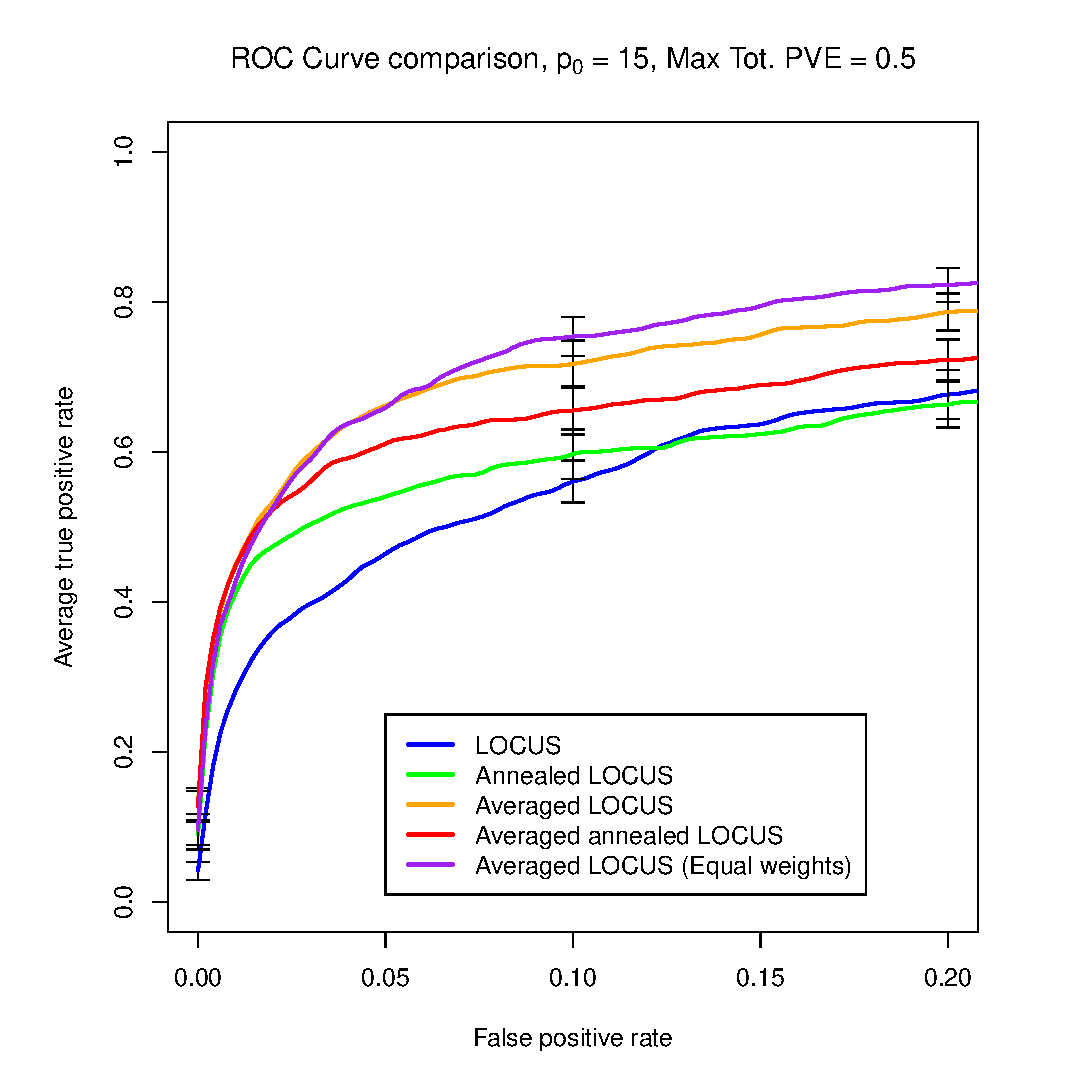
\includegraphics[width=2.8in, bb= 0 0 7.24in 7.24in]{images/ROC_15_05_095_099.pdf}
\put(-190,190){A}
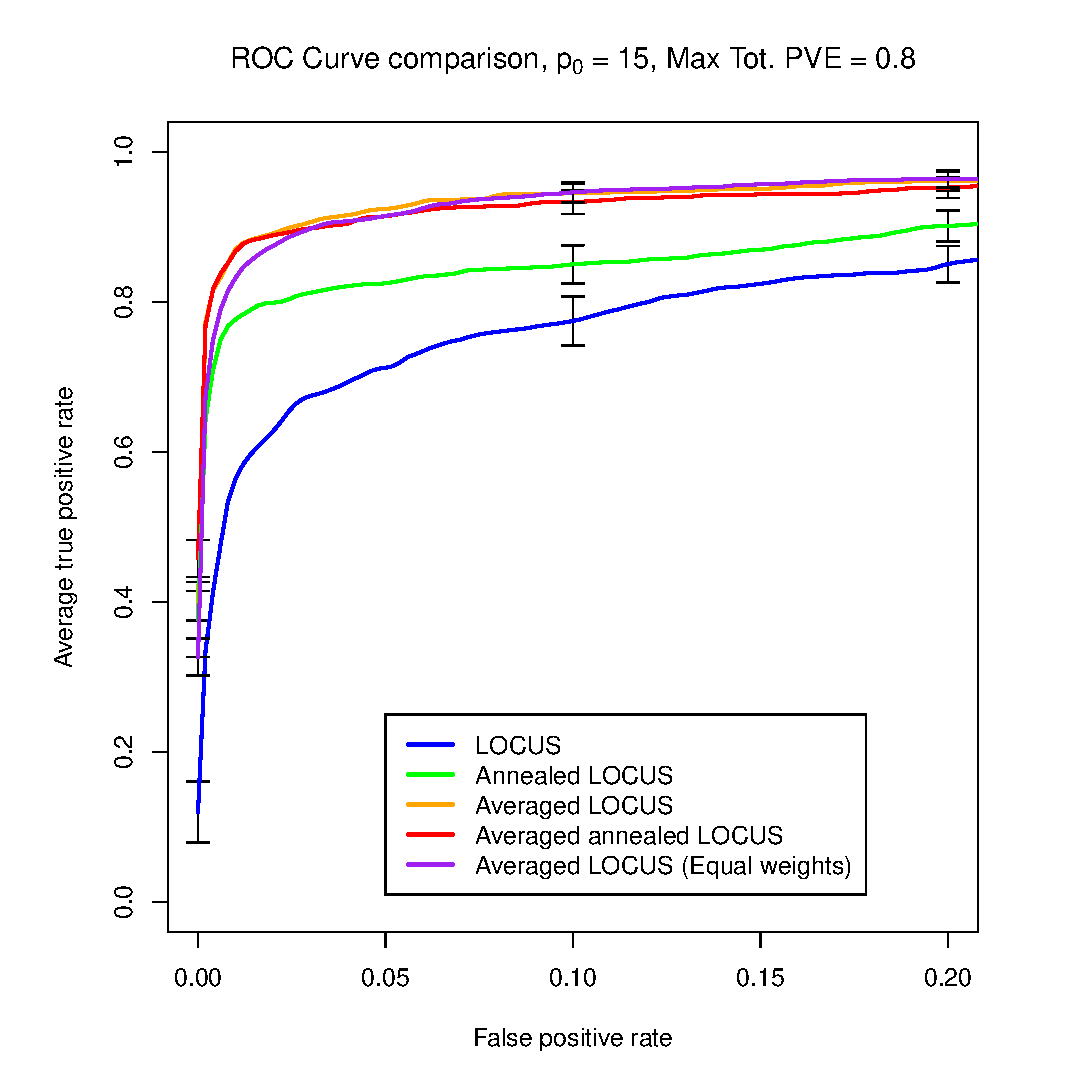
\includegraphics[width=2.8in, bb= 0 0 7.24in 7.24in]{images/ROC_15_08_095_099.pdf}
\put(-190,190){B}

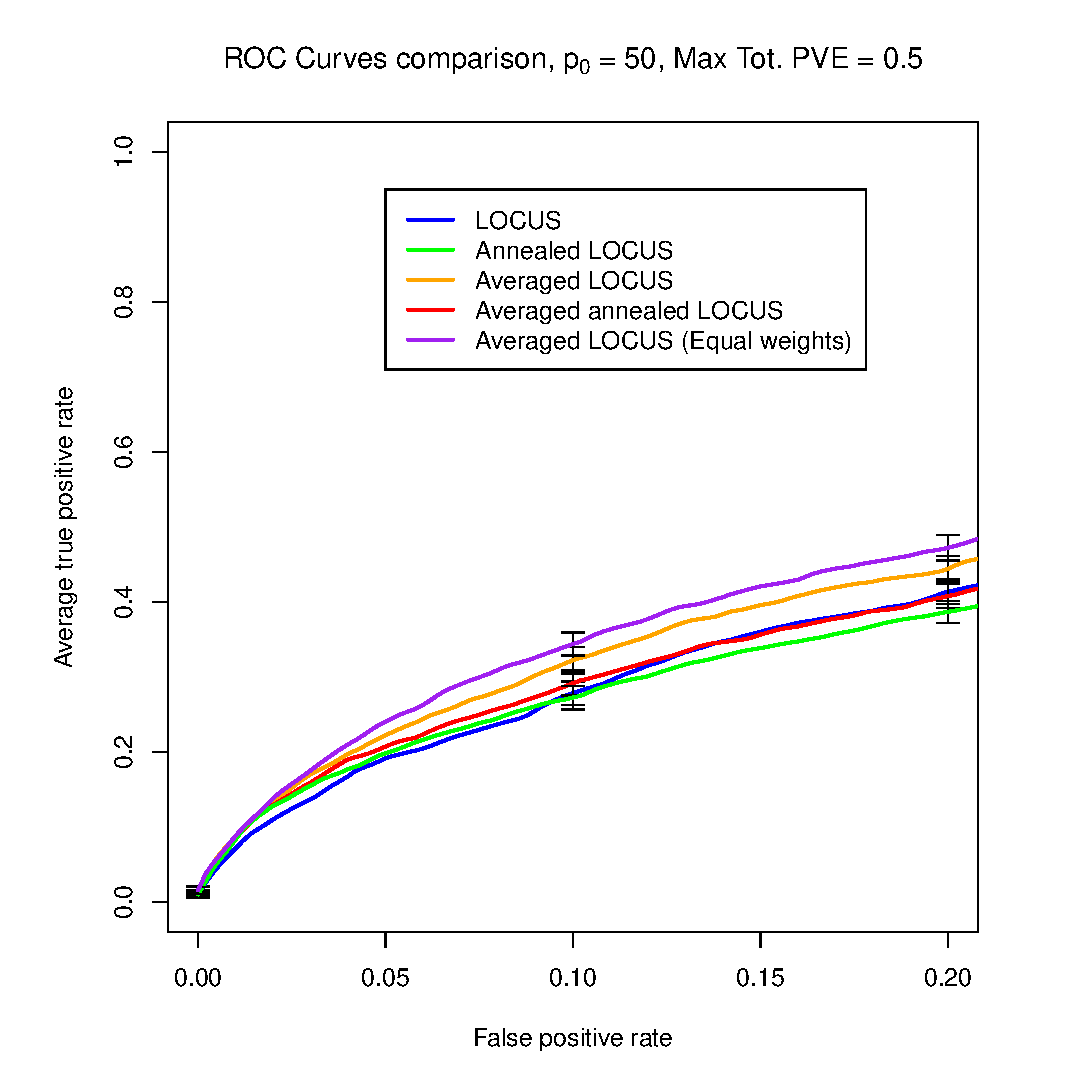
\includegraphics[width=2.8in, bb= 0 0 7.24in 7.24in]{images/ROC_50_05_095_099.pdf}
\put(-190,190){C}
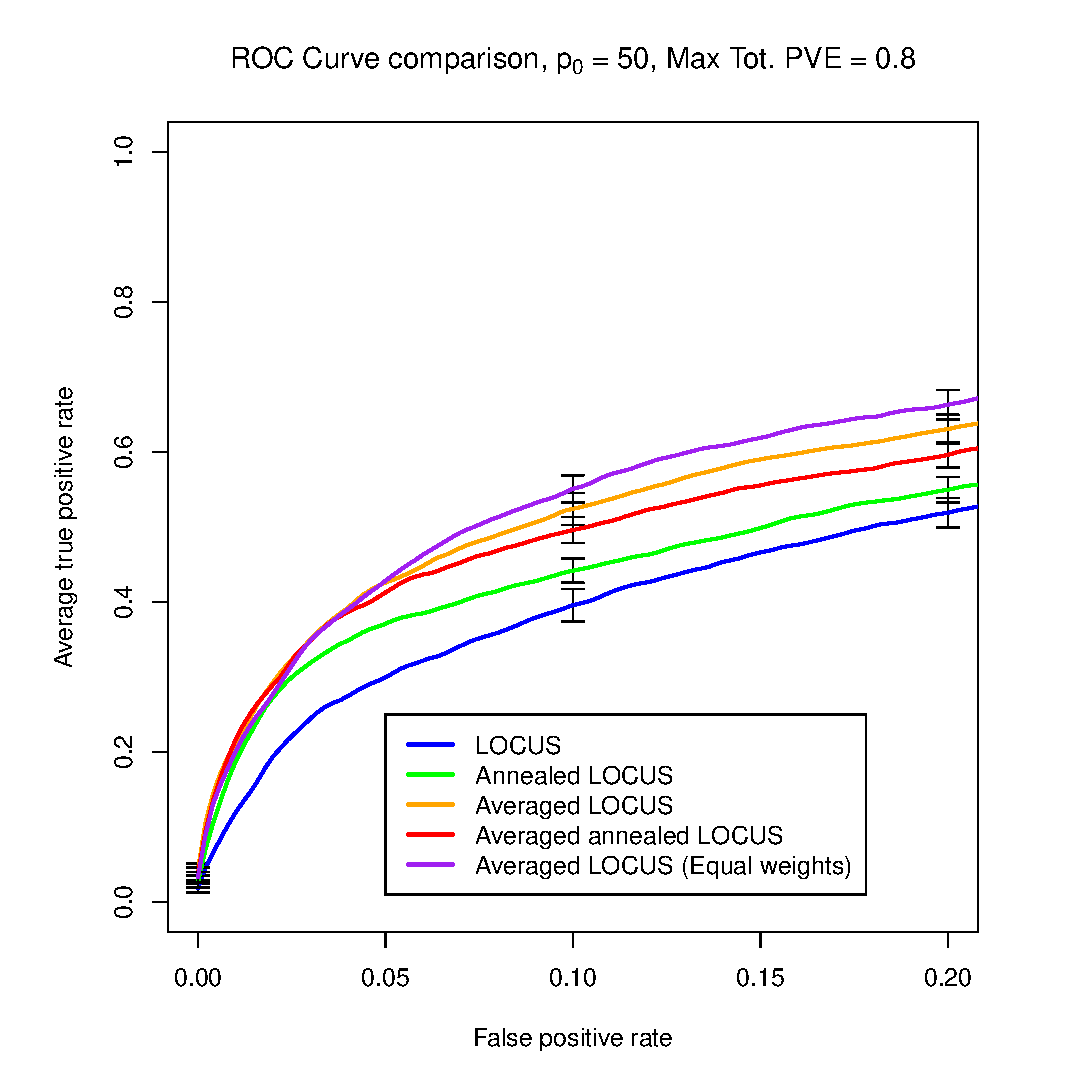
\includegraphics[width=2.8in, bb= 0 0 7.24in 7.24in]{images/ROC_50_08_095_099.pdf}
\put(-190,190){D}
\caption{\label{fig:ROC_highCorr}Comparison of ROC curves between LOCUS, averaged LOCUS, the same two methods augmented with a simulated annealing step, and averaged LOCUS with equal weights for every initialisation, colored orange, blue, red, green, and purple respectively. Top row: $15$ associated SNPs, Left column: maximum response variance $ = 0.5$,
Bottom row: $50$ associated SNPs, Right column: maximum response variance $ = 0.8$. The correlations between the SNPs are between $0.95$ and $0.99$.}
\end{figure}

Figure \ref{fig:ROC_highCorr} shows the variable selection performance in terms of ROC curves for the five methods, for each of the four settings. The correlations between the SNPs are high, between $0.95$ and $0.99$.

First, the averaged LOCUS method clearly outperforms the LOCUS method in all four scenarios: it seems that the weighted averaging procedure effectively alleviates the risk of selecting wrong predictors in groups of highly correlated SNPs.

Second, when starting both LOCUS and averaged LOCUS with a simulated annealing step, averaged LOCUS continues to be more powerful than LOCUS, although the improvement is smaller than without simulated annealing. This suggests that the annealing step does not prevent the averaged LOCUS algorithm from selecting multiple different models, in this strongly correlated data scenario. This could be because the chosen initial temperature is not sufficiently high to smooth the densities enough to access the right modes.

Third, annealed LOCUS outperforms LOCUS. The simulated annealing step allows the method to reach modes that cannot be reached by the LOCUS method with certain starting parameters. 

Fourth, in the less sparse setting with $50\%$ of variance explained by the predictors (setting C), the simulated effect sizes are weaker and all methods show similar, lower, performances: the averaging or annealing procedures do not lead to much improvement.

Fifth, averaging over all the modes, considering all weights to be equal, seems to perform better than averaged LOCUS. Figure \ref{fig:weightsModes} shows the weights attributed to each mode obtained by the averaged LOCUS method in setting A. More than half of the modes are attributed a weight equal to zero in the weighted average. Most of the modes are discarded in the averaged LOCUS method when they might have interesting information. Throughout the hundred initialisations, $62$ different SNPs have been attributed a probability of association bigger than $0.8$. The weights being based on an approximation of the log-likelihood $\log p(\boldsymbol{y}\mid M_k)$, $M_k$ designating the model obtained from the $k^{\mathrm{th}}$ initialisation, if said model estimates that only a single SNP is active, then the likelihood will be very small, and $\mathcal{L}(q)$ will be nearly zero. This mode will not be considered in the averaged LOCUS, but it will be considered when we consider all weights to be equal.

\begin{figure}[h!]
\centering
\includegraphics[width=5in]{images/Weights_Mode.pdf}
\caption{\label{fig:weightsModes}Weights attributed to the $100$ modes obtained by averaged LOCUS, with correlations between SNPs between $0.95$ and $0.99$, $15$ associated SNPs, and a proportion of the response variance explained by the SNPs below $50\%$.}
\end{figure}

Finally, averaged annealed LOCUS performs similarly to averaged LOCUS: their confidence intervals overlap. In setting A, averaged annealed LOCUS might even be less powerful: the simulated annealing step might diminish the number of modes considered for the average, putting more weight on wrong models.

\begin{figure}[h!]
\centering
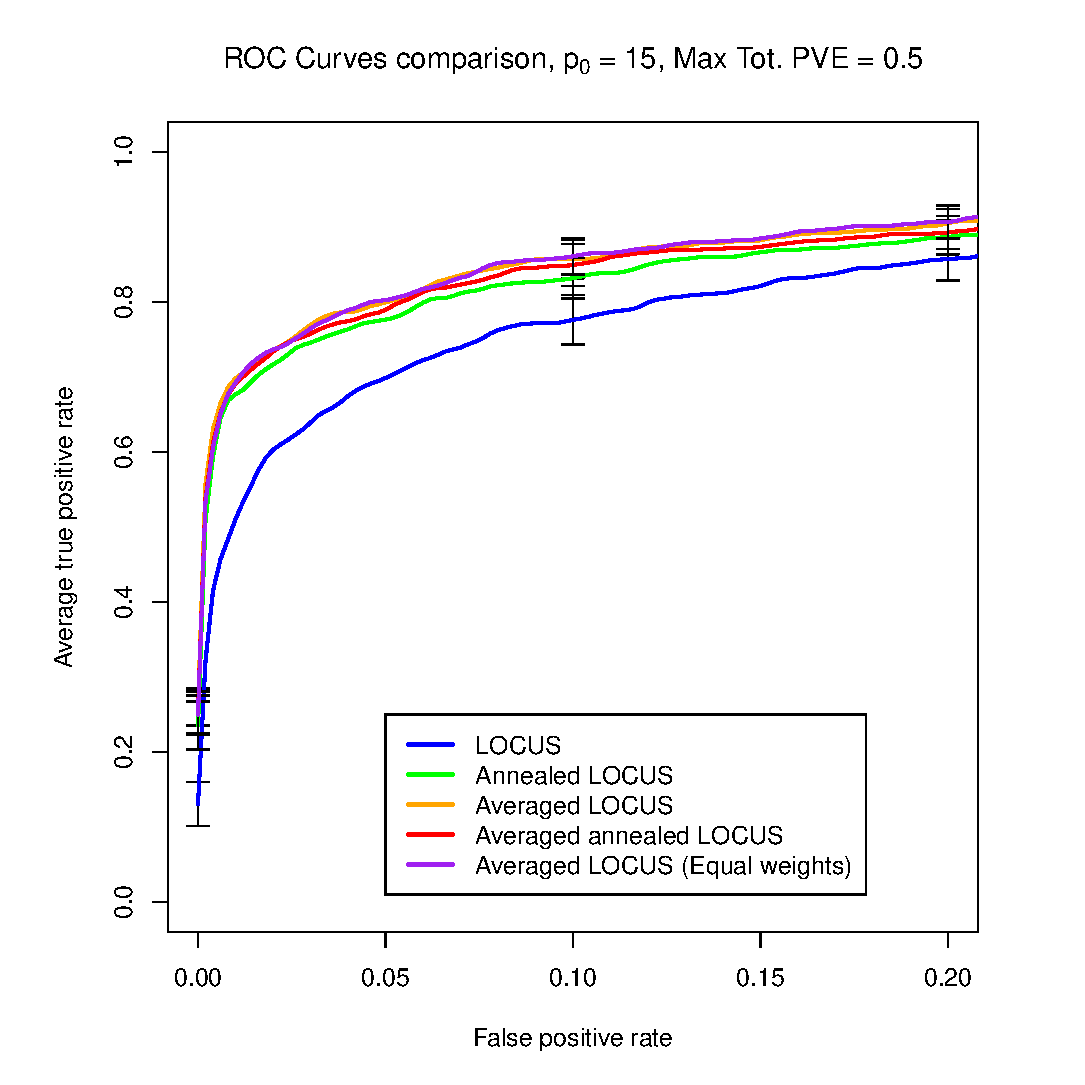
\includegraphics[width=2.8in, bb= 0 0 7.24in 7.24in]{images/ROC_15_05_07_095.pdf}
\put(-190,190){A}
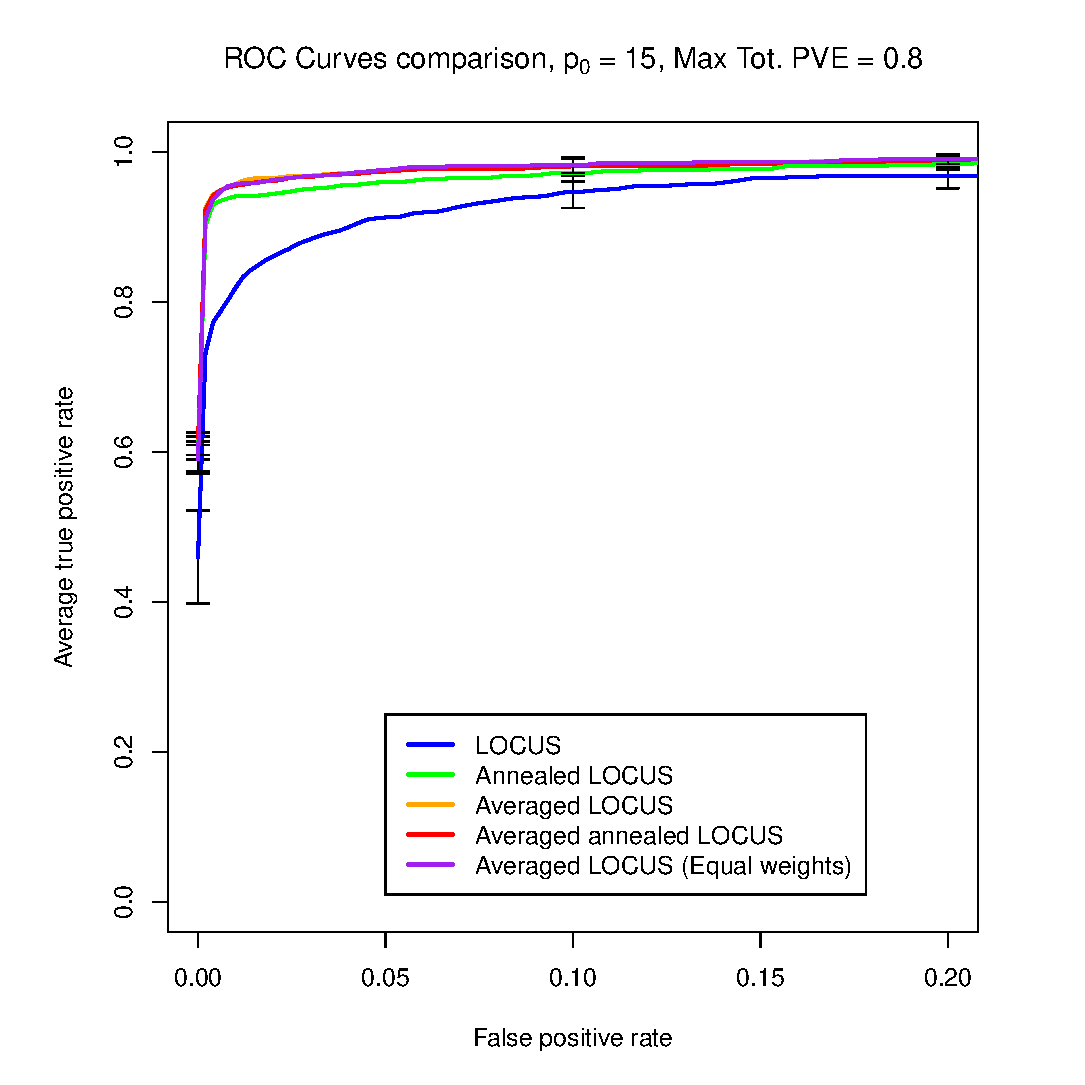
\includegraphics[width=2.8in, bb= 0 0 7.24in 7.24in]{images/ROC_15_08_07_095.pdf}
\put(-190,190){B}

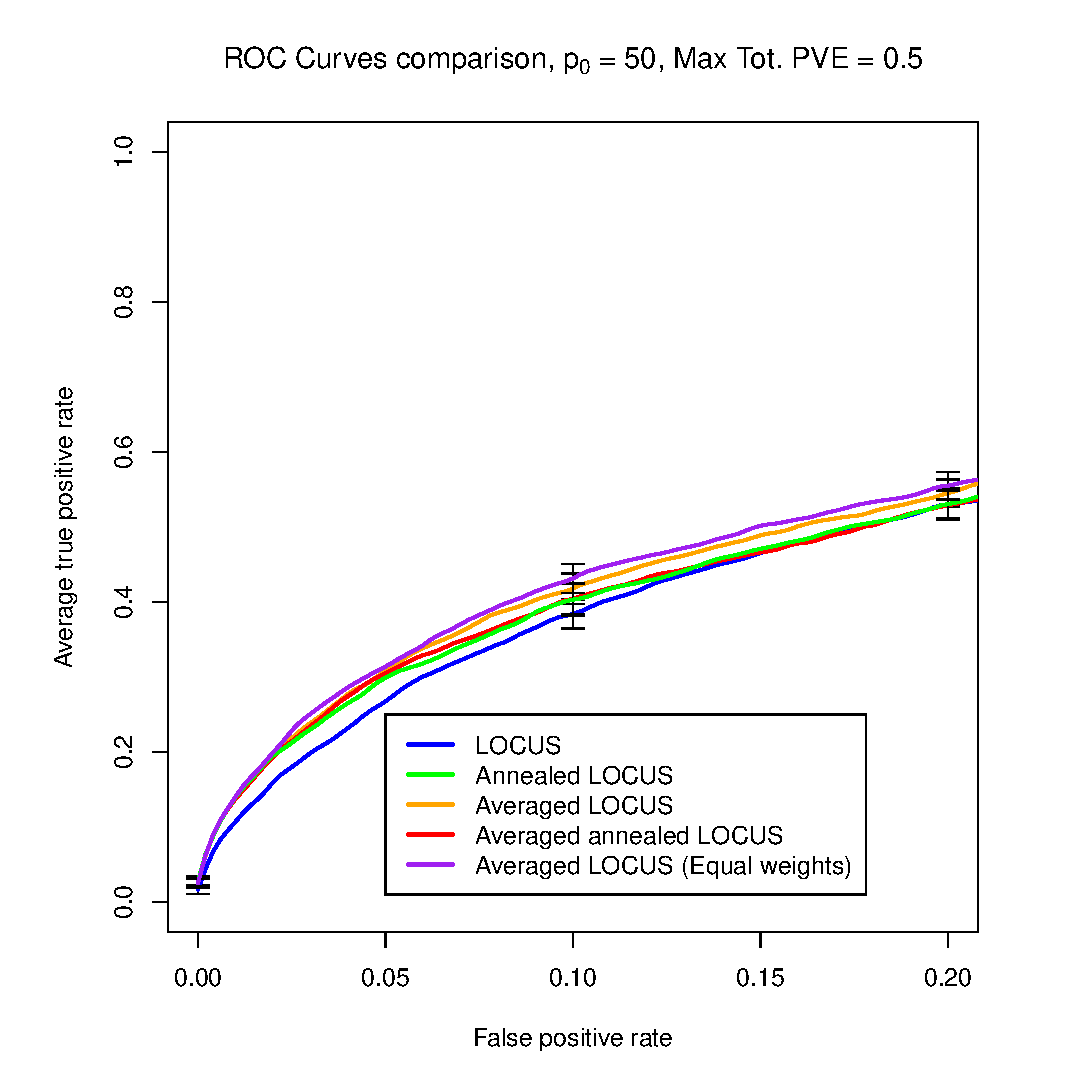
\includegraphics[width=2.8in, bb= 0 0 7.24in 7.24in]{images/ROC_50_05_07_095.pdf}
\put(-190,190){C}
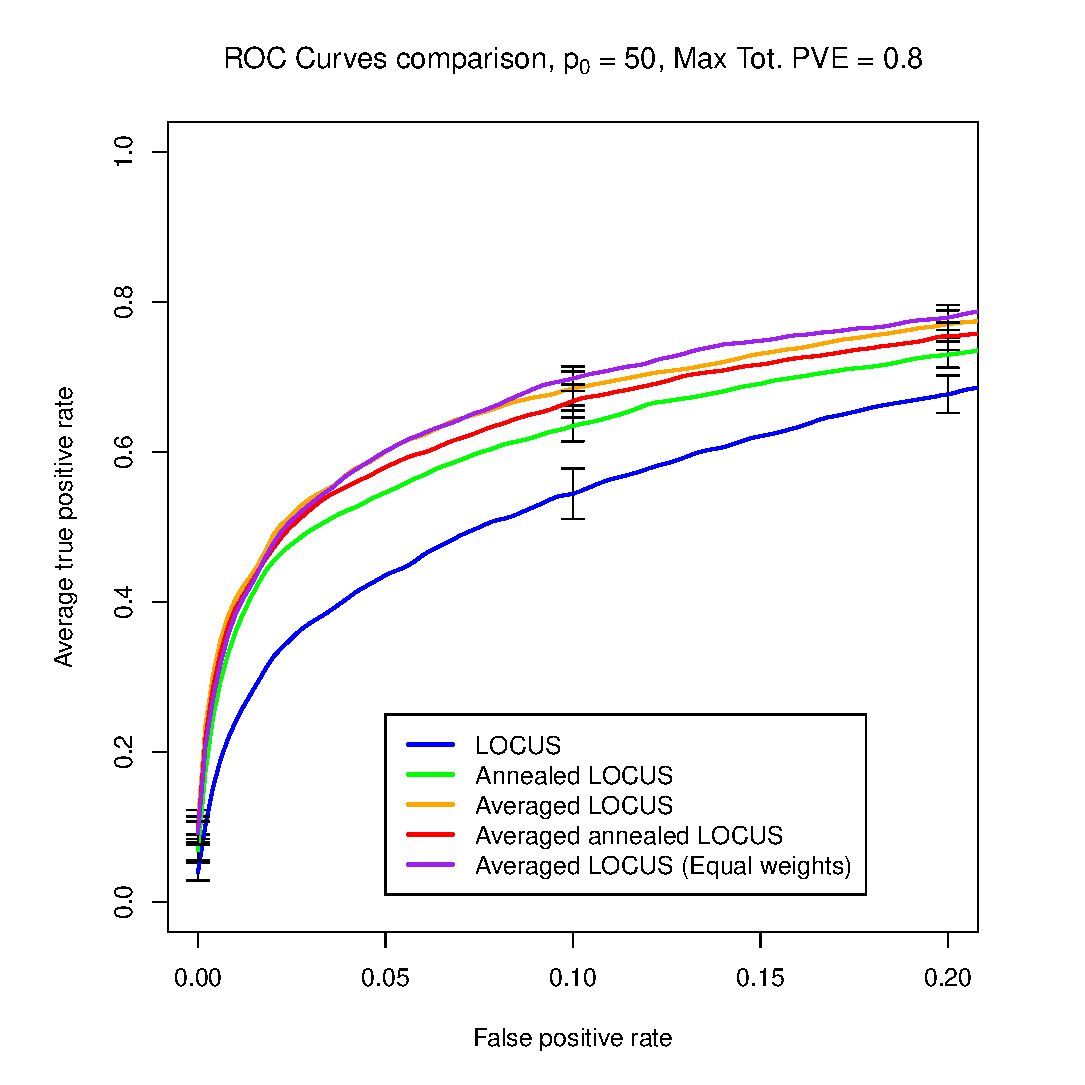
\includegraphics[width=2.8in, bb= 0 0 7.24in 7.24in]{images/ROC_50_08_07_095.pdf}
\put(-190,190){D}
\caption{\label{fig:ROC_mediumCorr}Comparison of ROC curves between LOCUS, averaged LOCUS, the same two methods augmented with a simulated annealing step, and averaged LOCUS with equal weights for every initialisation, colored orange, blue, red, green, and purple respectively. Top row: $15$ associated SNPs, Left column: maximum response variance $ = 0.5$,
Bottom row: $50$ associated SNPs, Right column: maximum response variance $ = 0.8$. The correlations between the SNPs are between $0.7$ and $0.95$.}
\end{figure}

Figure \ref{fig:ROC_mediumCorr} shows the variable selection performance in terms of the ROC curves for the five methods, for the same settings (A, B, C, D) than for Figure \ref{fig:ROC_highCorr}. The correlations between the SNPs are between $0.7$ and $0.95$.

First, LOCUS is outperformed by the four other methods in settings A, B, and D. In setting C, the five methods seem to perform similarly. The correlations seem to be high enough to mislead LOCUS, but low enough that averaging over multiple modes does not perform better than annealing LOCUS, i.e., finding a single mode.

Second, annealed LOCUS performs better than LOCUS in all settings, the annealing helps the method find a more suitable mode. However, in setting C, their performance is similar. The simulated effect sizes are weaker and all methods show lower performances, the multimodality of the posterior must be such that the annealing does not have a strong impact on the optimization quality.

Finally, averaged LOCUS, with or without equal weights, annealed LOCUS, and averaged annealed LOCUS perform similarly in all settings. The correlation between the SNPs is weak enough so that annealing LOCUS has a comparable variable selection performance as averaged LOCUS and averaged annealed LOCUS. 

\begin{figure}[h!]
\centering
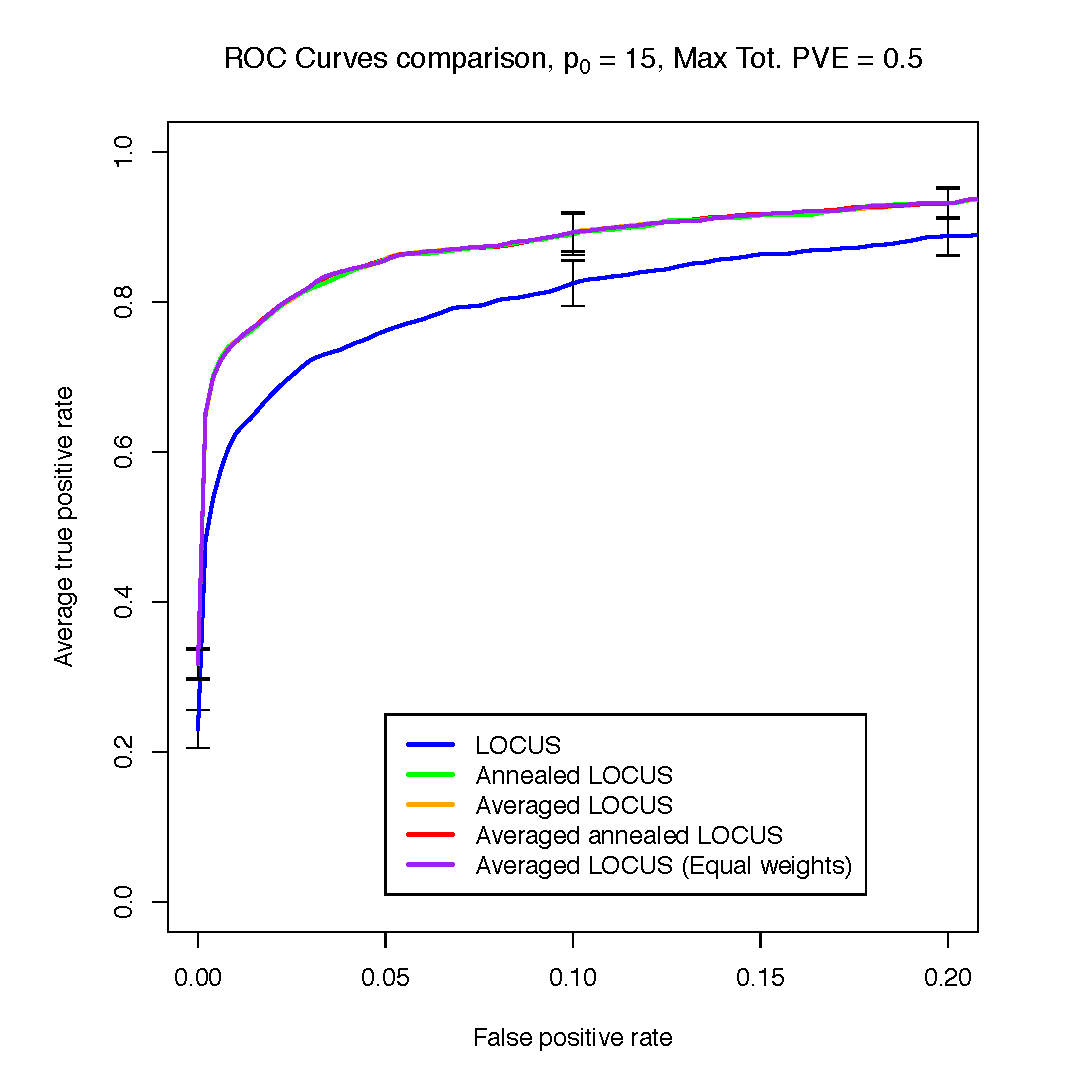
\includegraphics[width=2.8in, bb= 0 0 7.24in 7.24in]{images/ROC_15_05_05_07.pdf}
\put(-190,190){A}
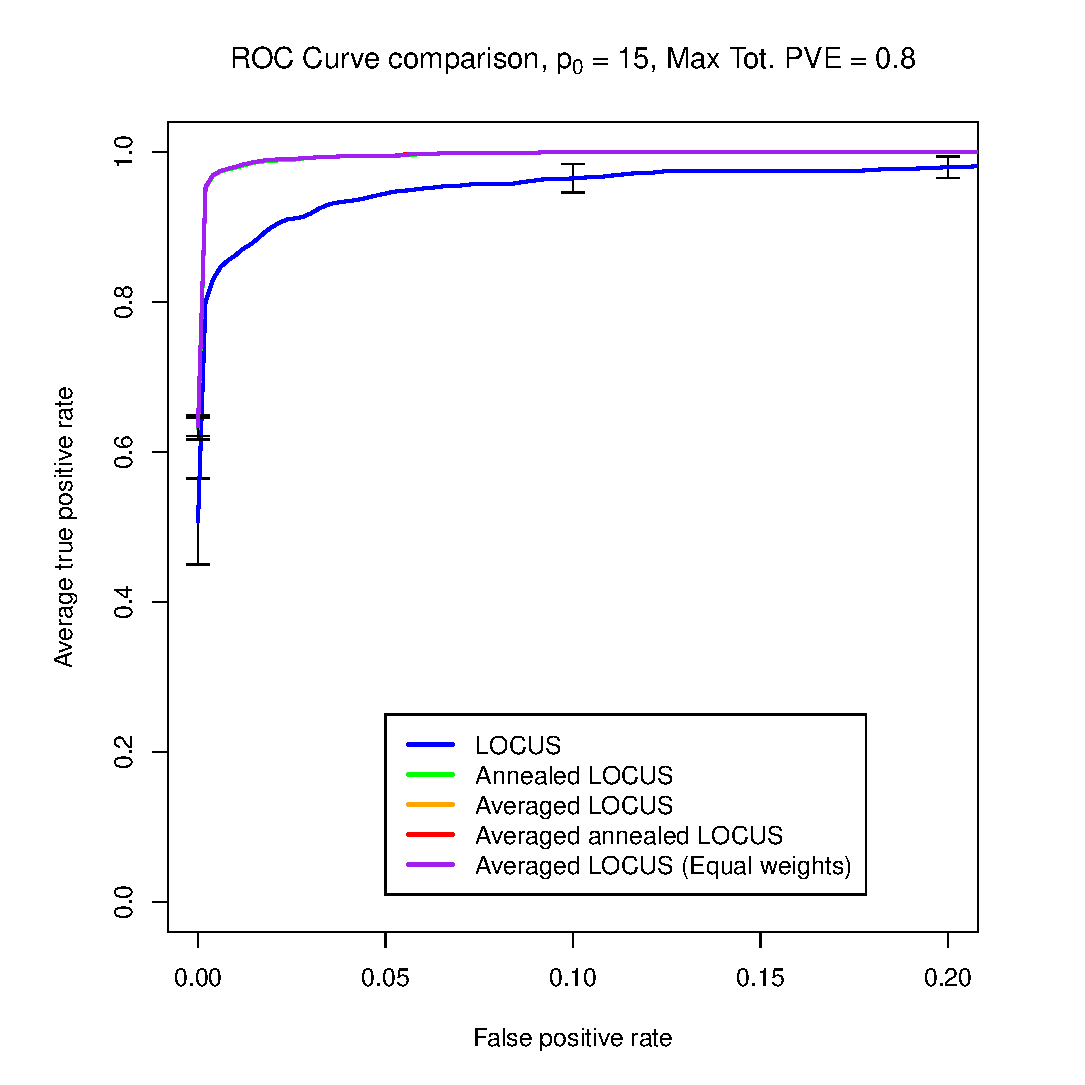
\includegraphics[width=2.8in, bb= 0 0 7.24in 7.24in]{images/ROC_15_08_05_07.pdf}
\put(-190,190){B}

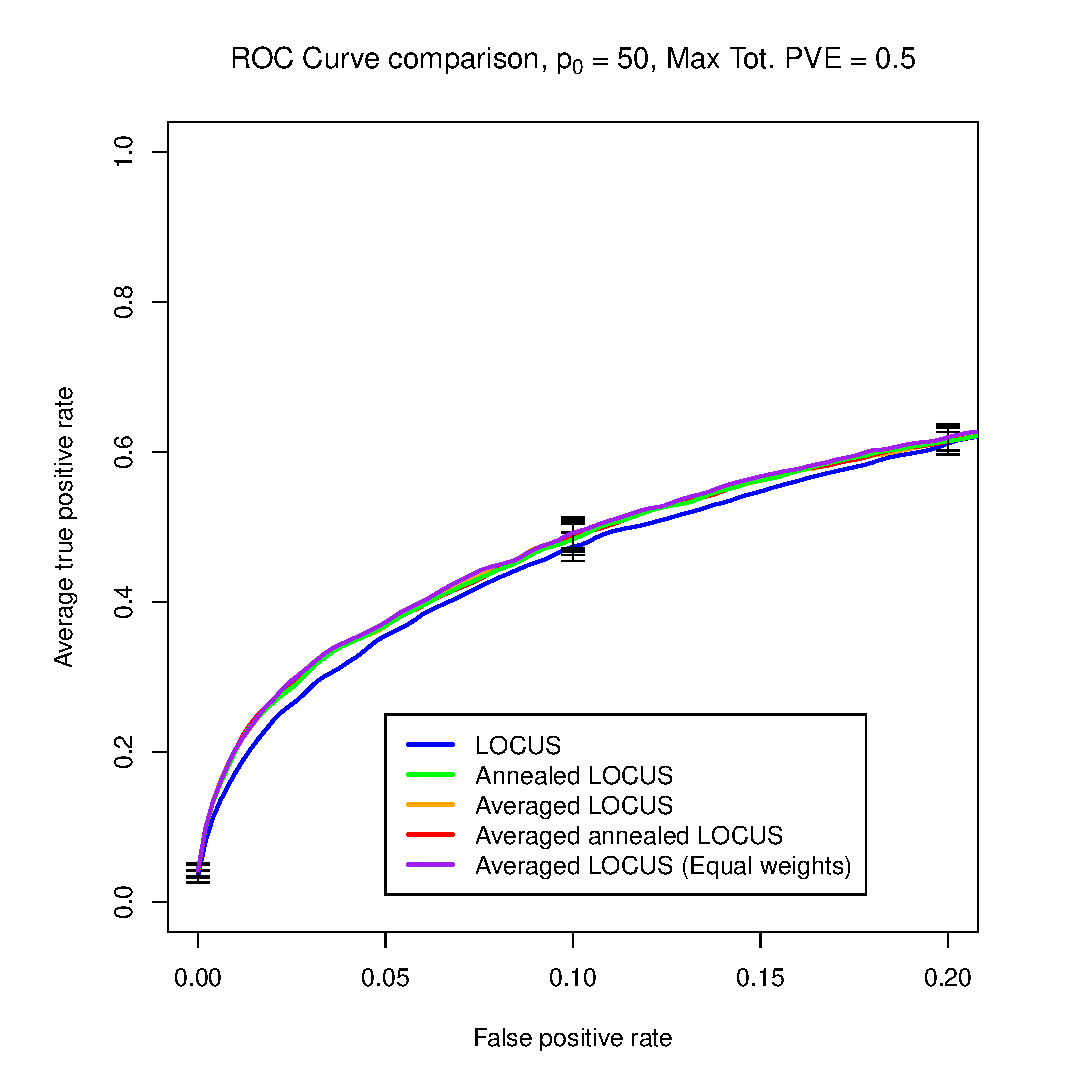
\includegraphics[width=2.8in, bb= 0 0 7.24in 7.24in]{images/ROC_50_05_05_07.pdf}
\put(-190,190){C}
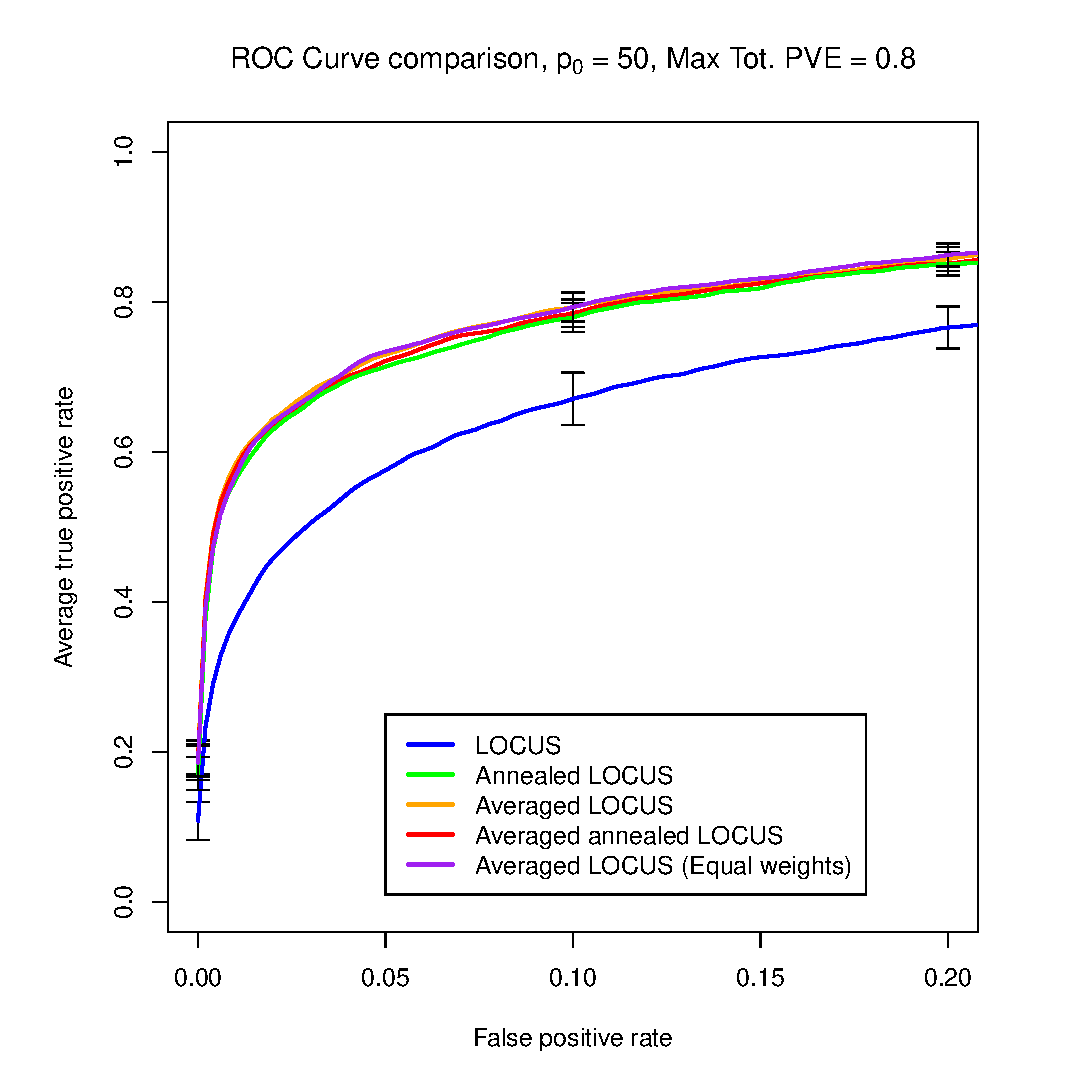
\includegraphics[width=2.8in, bb= 0 0 7.24in 7.24in]{images/ROC_50_08_05_07.pdf}
\put(-190,190){D}
\caption{\label{fig:ROC_lowCorr}Comparison of ROC curves between LOCUS, averaged LOCUS, the same two methods augmented with a simulated annealing step, and averaged LOCUS with equal weights for every initialisation, colored orange, blue, red, green, and purple respectively. Top row: $15$ associated SNPs, Left column: maximum response variance $ = 0.5$,
Bottom row: $50$ associated SNPs, Right column: maximum response variance $ = 0.8$. The correlations between the SNPs are between $0.5$ and $0.7$.}
\end{figure}

Figure \ref{fig:ROC_lowCorr} shows the ROC curves, representing the variable selection performance of the five methods, for the four settings (A, B, C, D), as in Figure \ref{fig:ROC_highCorr}. The correlations between the SNPs are between $0.5$ and $0.7$.

LOCUS is outperformed by the other methods in settings A, B, and D, as in Figure \ref{fig:ROC_mediumCorr}. In setting C, the performances of averaged LOCUS, annealed LOCUS, averaged annealed LOCUS, and averaged LOCUS with equal weights are indistinguishable. The correlations between the SNPs are weak enough for the four methods to perform similarly.

\begin{figure}[h!]
\centering
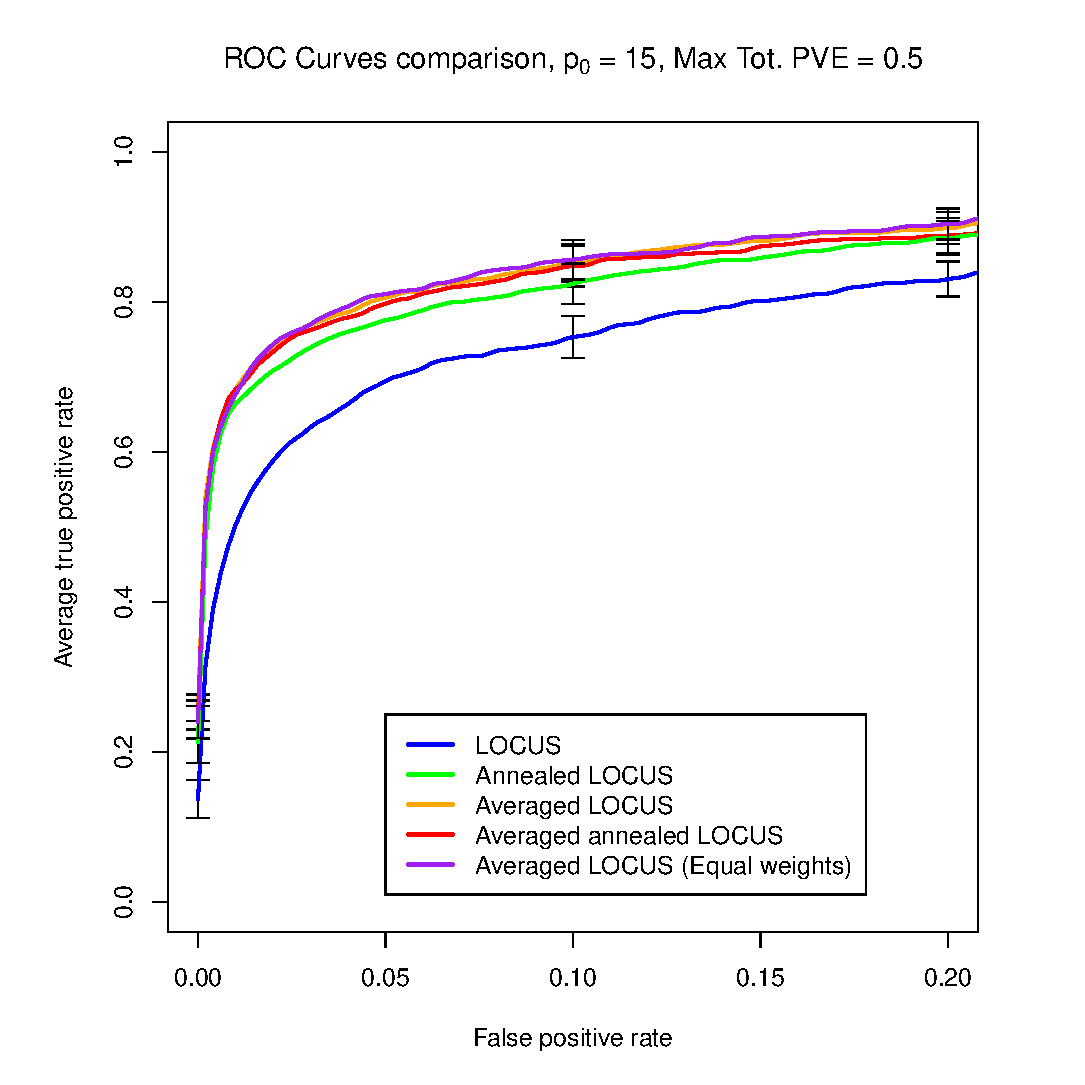
\includegraphics[width=2.8in, bb= 0 0 7.24in 7.24in]{images/ROC_15_05_05_099.pdf}
\put(-190,190){A}
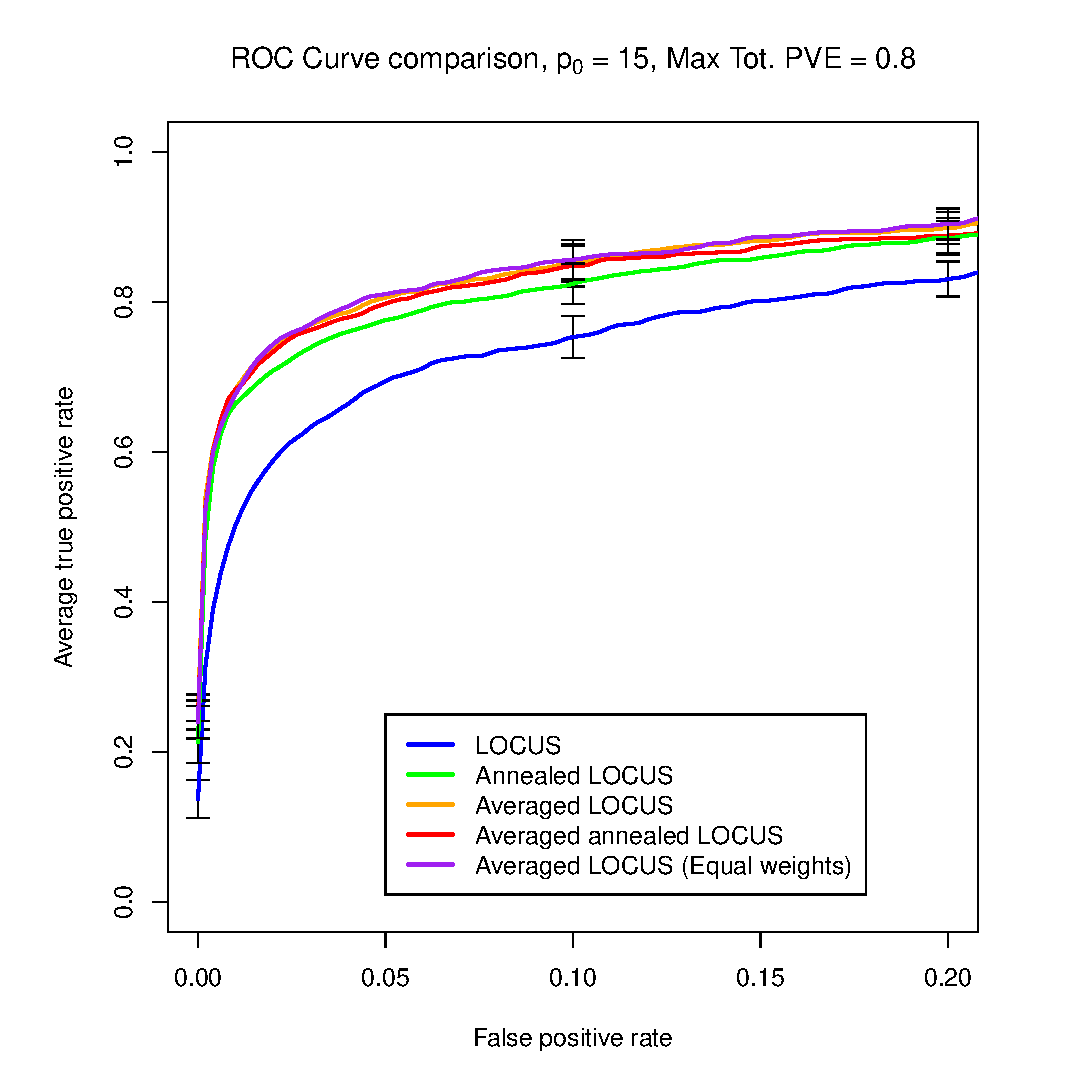
\includegraphics[width=2.8in, bb= 0 0 7.24in 7.24in]{images/ROC_15_08_05_099.pdf}
\put(-190,190){B}

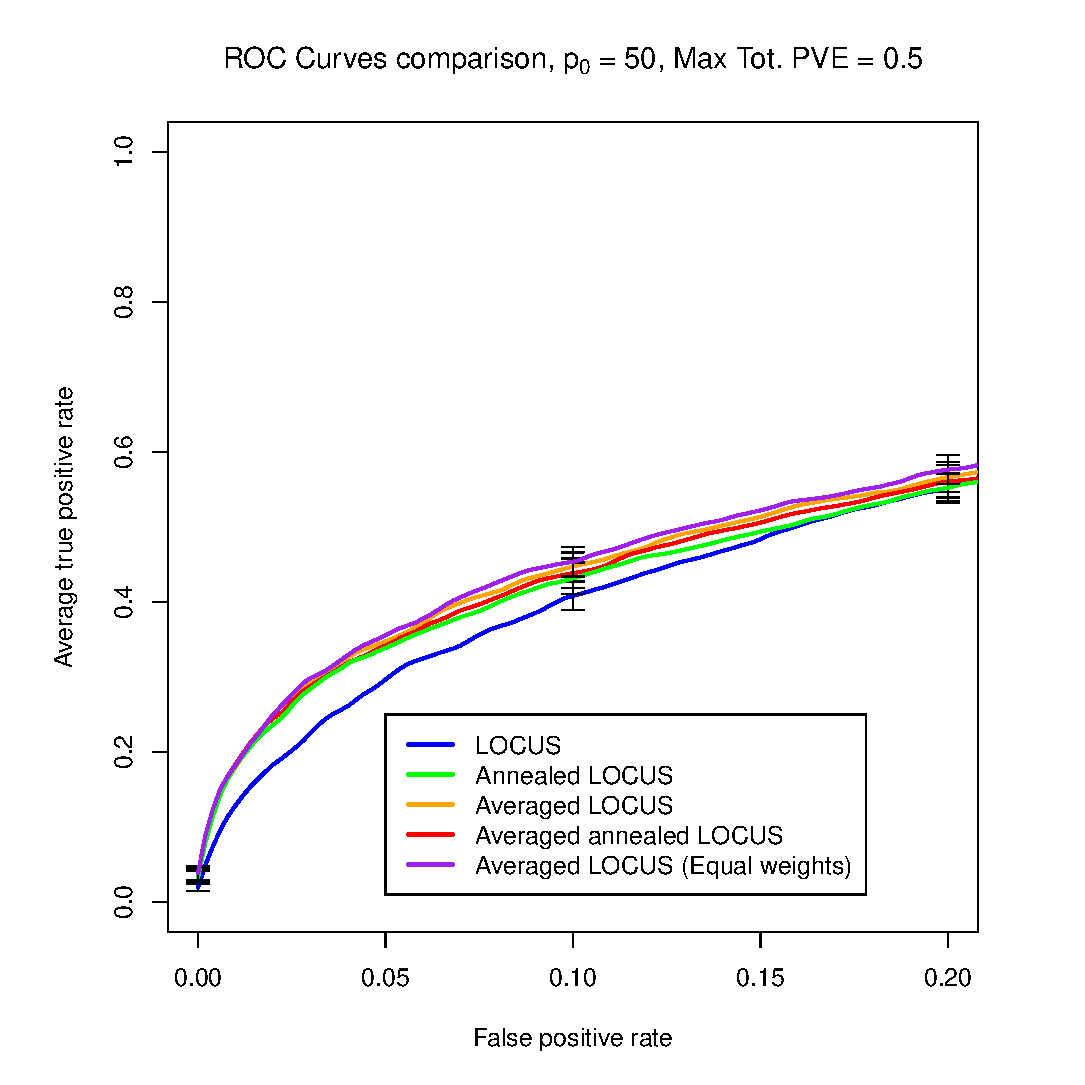
\includegraphics[width=2.8in, bb= 0 0 7.24in 7.24in]{images/ROC_50_05_05_099.pdf}
\put(-190,190){C}
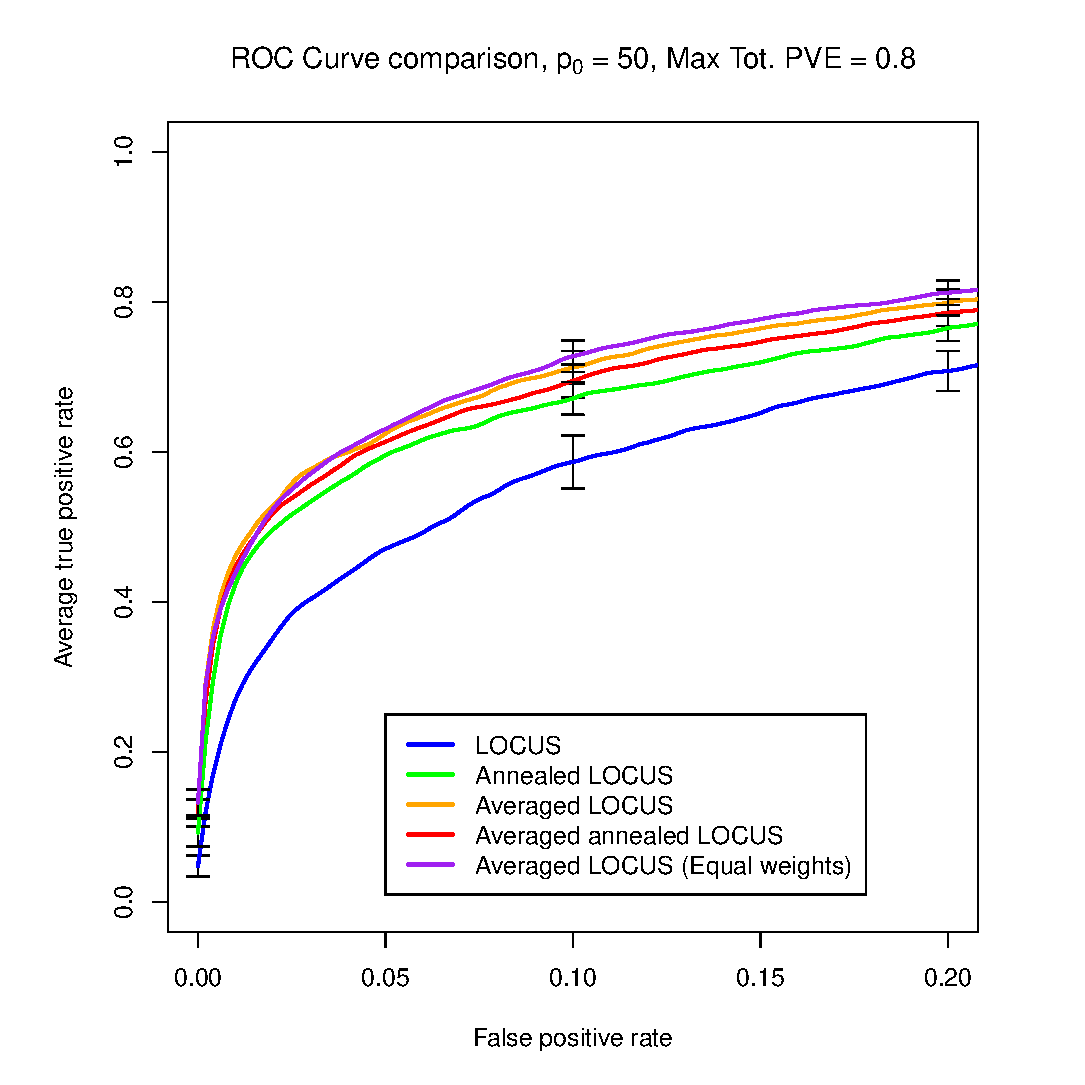
\includegraphics[width=2.8in, bb= 0 0 7.24in 7.24in]{images/ROC_50_08_05_099.pdf}
\put(-190,190){D}
\caption{\label{fig:ROC_mixedCorr}Comparison of ROC curves between LOCUS, averaged LOCUS, the same two methods augmented with a simulated annealing step, and averaged LOCUS with equal weights for every initialisation, colored orange, blue, red, green, and purple respectively. Top row: $15$ associated SNPs, Left column: maximum response variance $ = 0.5$,
Bottom row: $50$ associated SNPs, Right column: maximum response variance $ = 0.8$. The correlations between the SNPs are between $0.5$ and $0.99$.}
\end{figure}

Figure \ref{fig:ROC_mixedCorr} shows variable selection performances as ROC curves for the five methods, in four settings (A, B, C, D). The correlations between the SNPs are between $0.5$ and $0.99$, representing a mixture of the three previous experiments. The correlations in Figure \ref{fig:ROC_highCorr} are extreme, we should have results closer to those of Figures \ref{fig:ROC_mediumCorr} and \ref{fig:ROC_lowCorr}.

LOCUS is outperformed by the four other methods in settings A, B, and D, but its performance seems to be similar to the four others in setting C. This goes with what we read in Figures \ref{fig:ROC_highCorr}, \ref{fig:ROC_mediumCorr}, and \ref{fig:ROC_lowCorr}.

Averaged LOCUS, with or without equal weights, annealed LOCUS, and averaged annealed LOCUS have similar performances. The weights do not improve the performance of the averaged LOCUS. These observations are similar to what we observed in Figures \ref{fig:ROC_mediumCorr} and  \ref{fig:ROC_lowCorr}. 

The correlations being between $0.5$ and $0.99$, they have a higher chance of being in the range of the correlations of Figures \ref{fig:ROC_mediumCorr} and \ref{fig:ROC_lowCorr} than being in the range of the correlations of Figure \ref{fig:ROC_highCorr}. The performances on the mixed correlation settings being similar to the performances on the weak and medium correlation settings makes sense. 


\section{Comparison with MCMC inference} \label{sec:comparison}
Section \ref{sec:varSelPerf} evaluated variable selection performance of the different methods and we now check our proposal by confronting it with MCMC inference. To do so, we generate data with the \texttt{echoseq R}-package, and save the simulated matrix $\boldsymbol{\beta}$. We simulate $300$ observations of four equicorrelated SNPs with an extremely high correlation coefficient of $0.995$. Of the four SNPs, two are associated with a trait.

We compare the posterior distributions of the regression coefficient obtained by our methods with the posterior distributions obtained by MCMC inference. The two inference methods have a different convergence and stopping criteria, so the comparison should be studied prudently. Our method is based on variational inference, which has a convergence criterion defined as a tolerance to be given. The MCMC inference does not necessarily visit the whole model space, so to alleviate this problem, we run it for $10^5$ iterations and discard the first half as burn-in, and we consider a very small problem, i.e., $p=4, q=1$. We are interested in evaluating the posterior distributions of $\boldsymbol{\beta} = (\beta_1, \beta_2, \beta_3, \beta_4)$. In the construction of our data, we have chosen $\beta_2, \beta_3 = 0$ and $\beta_1, \beta_4 \neq 0$.
\begin{figure}[h]
\centering
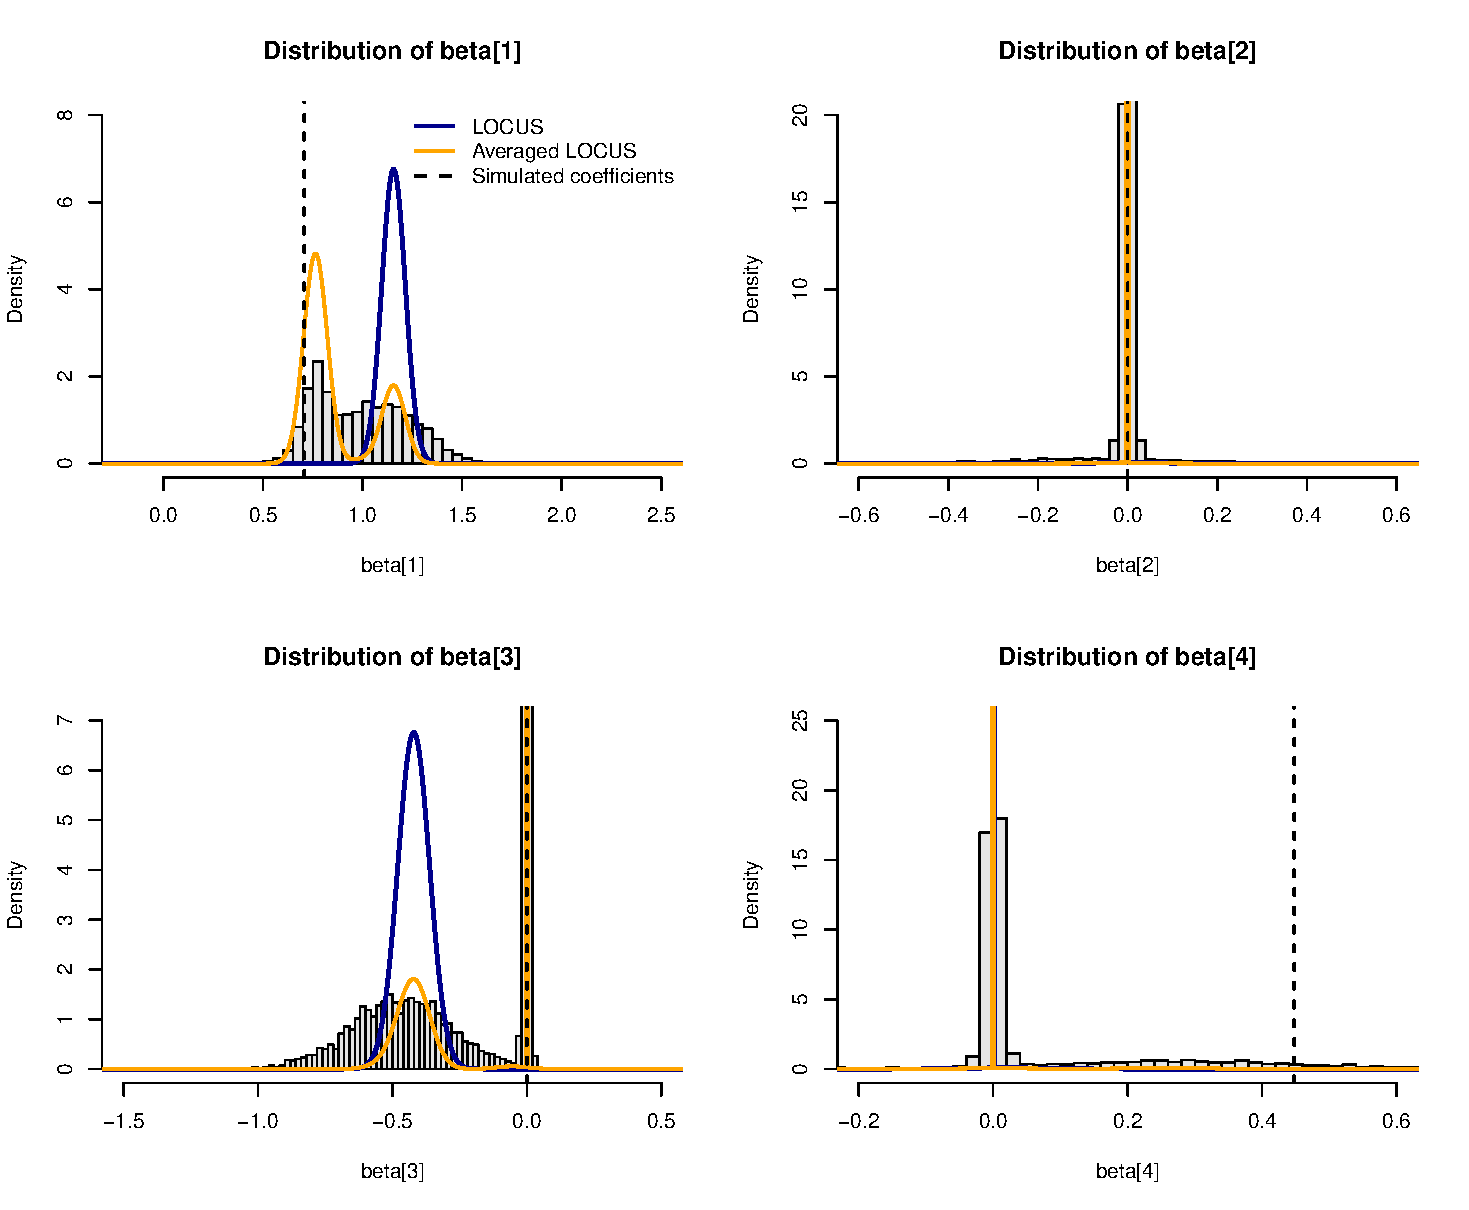
\includegraphics[width=\textwidth, bb=0 0 9.8in 8.07in]{images/MCMC_noanneal.pdf}
\caption{\label{fig:no_ann}Comparison of LOCUS (blue) and averaged LOCUS (orange) estimated posterior distributions for $\boldsymbol{\beta}$, MCMC distributions (histograms), as well as the simulated $\boldsymbol{\beta}$ values (dashed black line). The orange and blue lines of $\beta_2$ and $\beta_4$ are superimposed. The SNPs are equicorrelated with a correlation coefficient of $0.995$.}
\end{figure}

Figure \ref{fig:no_ann} shows LOCUS and averaged LOCUS estimated posteriors of $\boldsymbol{\beta}$, as well as the histograms of the MCMC posteriors and the simulated values of $\boldsymbol{\beta}$. 

First, the problem appears to be very difficult as all methods  fail to accurately capture the simulated values; even the MCMC algorithm yields inferences far from the truth for $\beta_4$. It is supposed to be non-null, but the MCMC approximations and those given by LOCUS and averaged LOCUS are all concentrated around zero. The correlations are too strong and the effect sizes are too weak for the algorithms to find the simulated $\beta_4$. To verify this, Figure \ref{fig:weakCorr} shows a case with weaker correlations and stronger effect sizes.

Second, averaged LOCUS probably best reflects the true posterior; it puts mass near the simulated values of $\beta_s$ for every $\beta_s$ but for $\beta_4$, where it finds the same estimate as the MCMC inference and the LOCUS methods. This is in line with the ROC curves of Figure \ref{fig:ROC_highCorr}, where we saw that for variable selection, averaged LOCUS outperforms LOCUS.

Third, when LOCUS and averaged LOCUS disagree, the result of LOCUS is ``visible'' in the distribution of averaged LOCUS. Averaged LOCUS considers the mode obtained from LOCUS in its averaging.

Finally, the shift between the simulated $\beta_1$ and the algorithms estimations is not expected. It is acceptable to have a shrinkage when estimating simulated values with inference, but the shift is supposed to be in the direction of zero. The algorithms MCMC, LOCUS, and averaged LOCUS having wrongly not selected the fourth SNP as associated, compensated on the first SNP. The observations $\boldsymbol{y}$ should follow $\boldsymbol{y} \sim \boldsymbol{X}\boldsymbol{\beta} + \boldsymbol{\varepsilon}$, with $\varepsilon$ the error, $\beta_2$ and $\beta_3$ equal to zero, $\beta_1$ and $\beta_2$ bigger than zero. If the algorithms estimate $\beta_2$, $\beta_3$, and $\beta_4$ to be equal to zero, then they will estimate $\beta_1$ to be bigger than what it is supposed to be.

\begin{figure}[h]
\centering
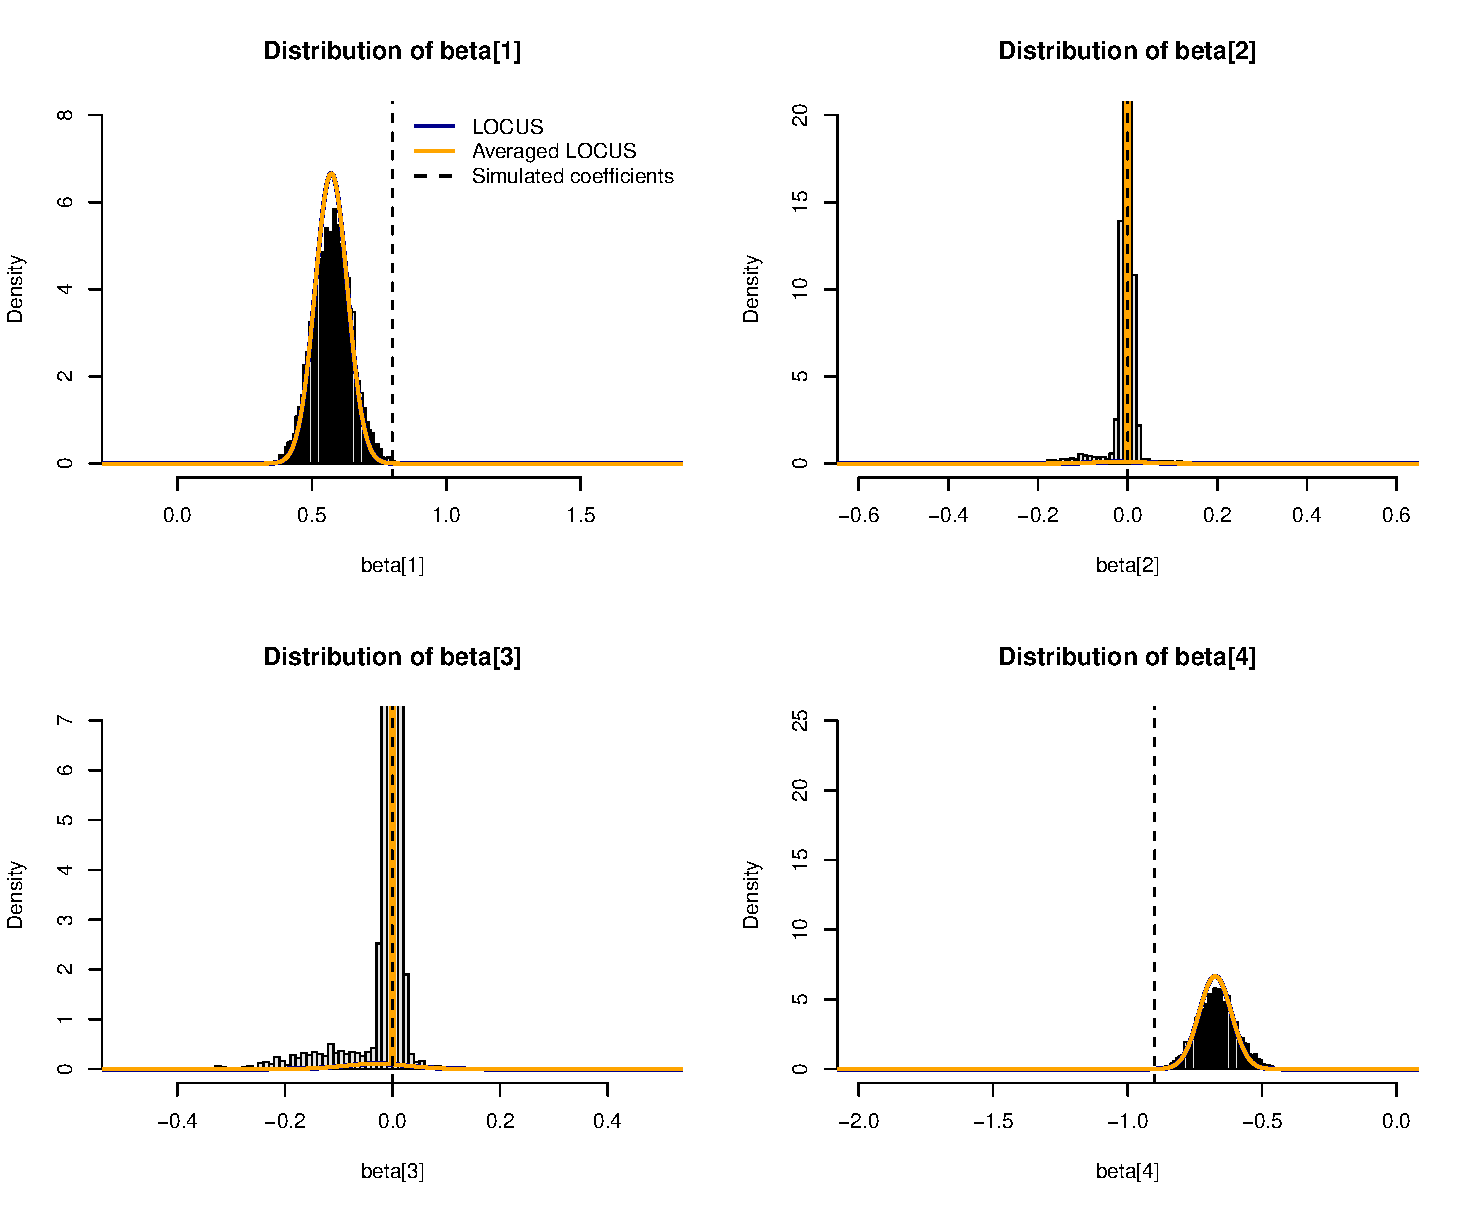
\includegraphics[width=\textwidth, bb=0 0 9.8in 8.07in]{images/MCMC_weakcorr.pdf}
\caption{\label{fig:weakCorr} Comparison of LOCUS (blue) and averaged LOCUS (orange) estimated posterior distributions for $\boldsymbol{\beta}$, MCMC distributions (histograms), as well as the simulated $\boldsymbol{\beta}$ values (dashed black line). The orange and blue lines are superimposed. The SNPs are autocorrelated with a correlation coefficient of $0.9$. The blue and orange lines are superimposed.}
\end{figure}

Figure \ref{fig:weakCorr} shows LOCUS and averaged LOCUS estimated posteriors of $\boldsymbol{\beta}$, the histograms of the MCMC posteriors, and the simulated values of $\boldsymbol{\beta}$, for SNPs autocorrelated with a correlation coefficient of $0.9$, weaker than for Figure \ref{fig:no_ann}, and a stronger effect size for $\beta_4$.

The weaker correlations and stronger effect size for $\beta_4$ allow the algorithms to better estimate the simulated effect sizes $\boldsymbol{\beta}$. The active SNPs have been correctly estimated, and the inactive SNPs have been detected.

LOCUS and averaged LOCUS yield similar posterior distributions for $\boldsymbol{\beta}$. Due to the correlation being weaker and the effect sizes being bigger, LOCUS can estimate the effect sizes just as well as averaged LOCUS does. 

\begin{figure}[h]
\centering
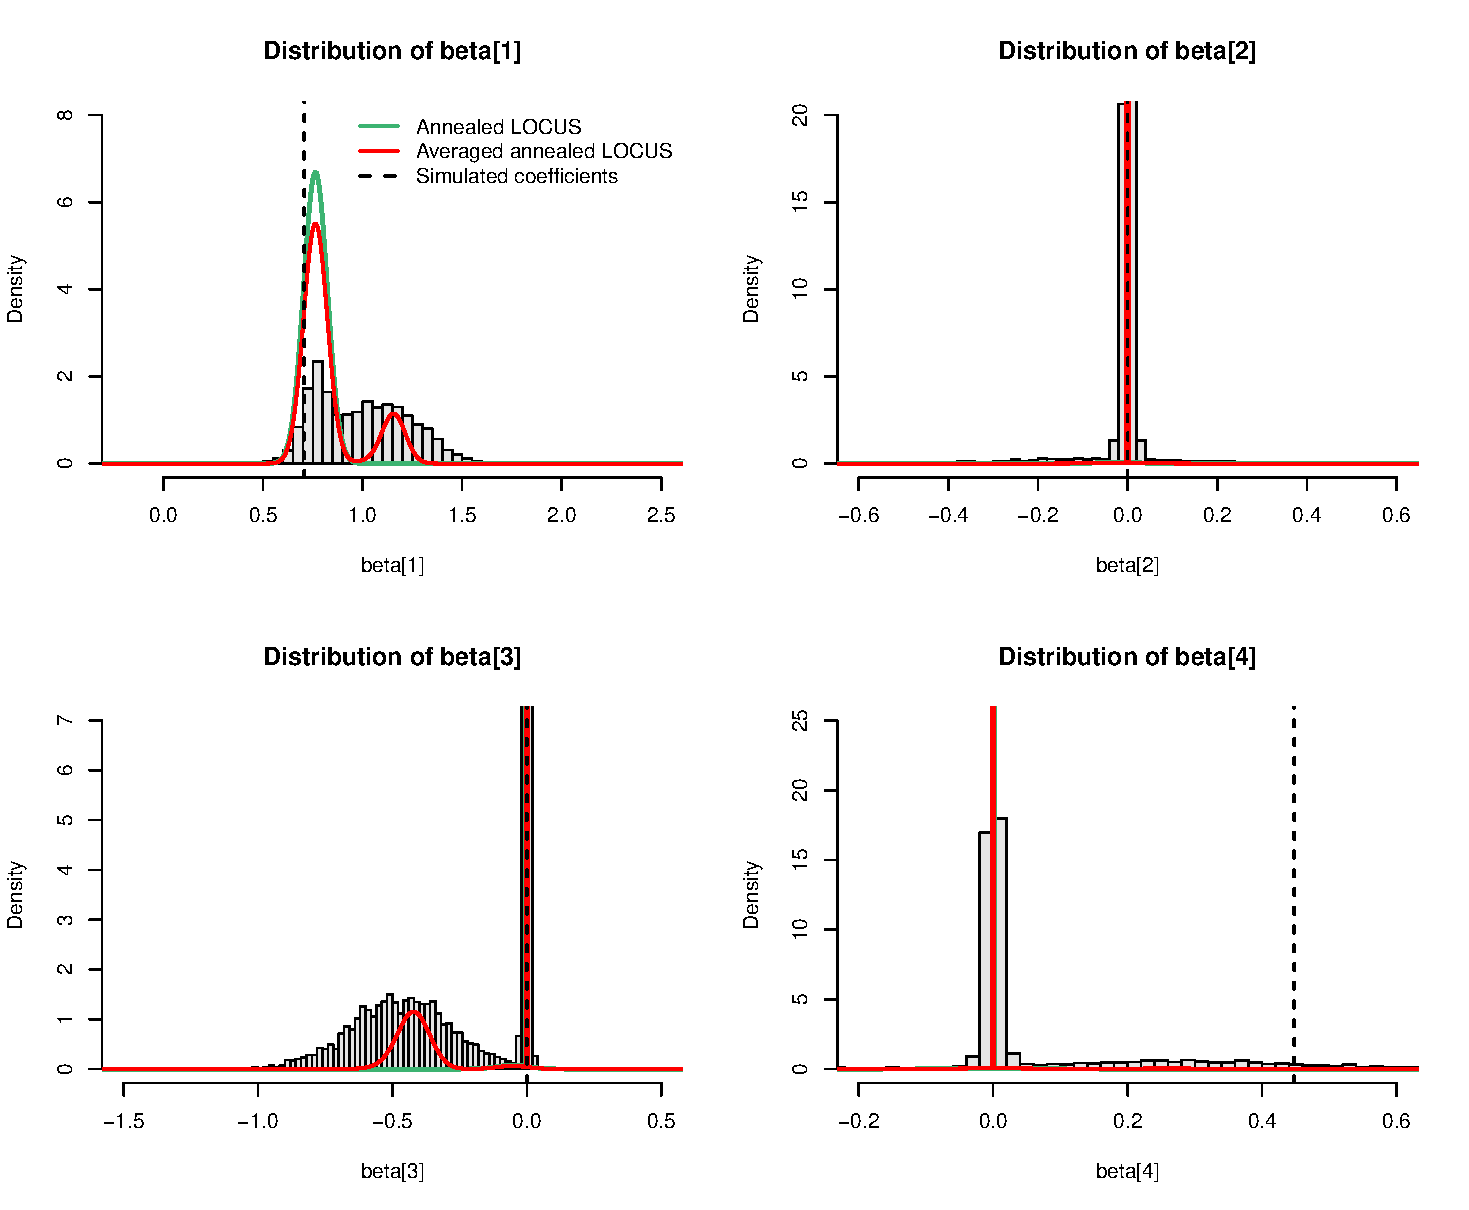
\includegraphics[width=\textwidth, bb=0 0 9.8in 8.07in]{images/MCMC_anneal.pdf}
\caption{\label{fig:ann}Comparison of annealed LOCUS (green) and averaged annealed LOCUS (red) estimated posterior distribution for $\boldsymbol{\beta}$, MCMC distributions (histograms) $\boldsymbol{\beta}$ posteriors and the simulated $\boldsymbol{\beta}$ values (dashed black line). The SNPs are equicorrelated with a correlation coefficient of $0.995$.}
\end{figure}

Figure \ref{fig:ann} shows the same posteriors as Figure \ref{fig:no_ann}, but with a simulated annealing step added to the LOCUS and averaged LOCUS methods. We have used the same settings than for Figure \ref{fig:no_ann}, so the histograms and the simulated $
\boldsymbol{\beta}$ values are the same for the two situations. We chose an initial temperature $T_L = 5$, and used ten geometric steps.

For all four $\beta_s$, annealed LOCUS yields a posterior density that is aligned with averaged annealed LOCUS. The posterior given by annealed LOCUS tends to put mass at the same place as the averaged annealed LOCUS posterior.

As for the non annealing methods, the simulated annealing augmented methods overlap the simulated values for all $\beta_s$ except for $\beta_4$ where, the MCMC simulation and the augmented methods yield a posterior with values concentrated around zero. As for Figure \ref{fig:no_ann}, the correlations were too strong and the effect sizes too weak for the algorithms to find a suitable estimation for $\beta_4$. And in the same way as in Figure \ref{fig:no_ann}, the fourth SNP not being recognised as associated, the algorithms must have compensated on the first SNP, overestimating its effect size $\beta_1$.

When comparing the plots of Figures \ref{fig:no_ann} and \ref{fig:ann}, one sees that the annealing changed the posterior densities. In Figure \ref{fig:no_ann}, the posterior densities of the LOCUS method for $\beta_1$ and $\beta_3$ were putting weight on different mode than averaged LOCUS, but in Figure \ref{fig:ann} the posterior density of the annealed LOCUS method put weight in the same places the averaged annealed LOCUS has the most weight. 

\section{Running times}

Our method, whether with simulated annealing or not, can be implemented in parallel, which can drastically diminish the runtime. Even if the method has to wait until the last run to converge, we would still be quicker than calculating the runs one after the other.

\begin{figure}[h]
\centering
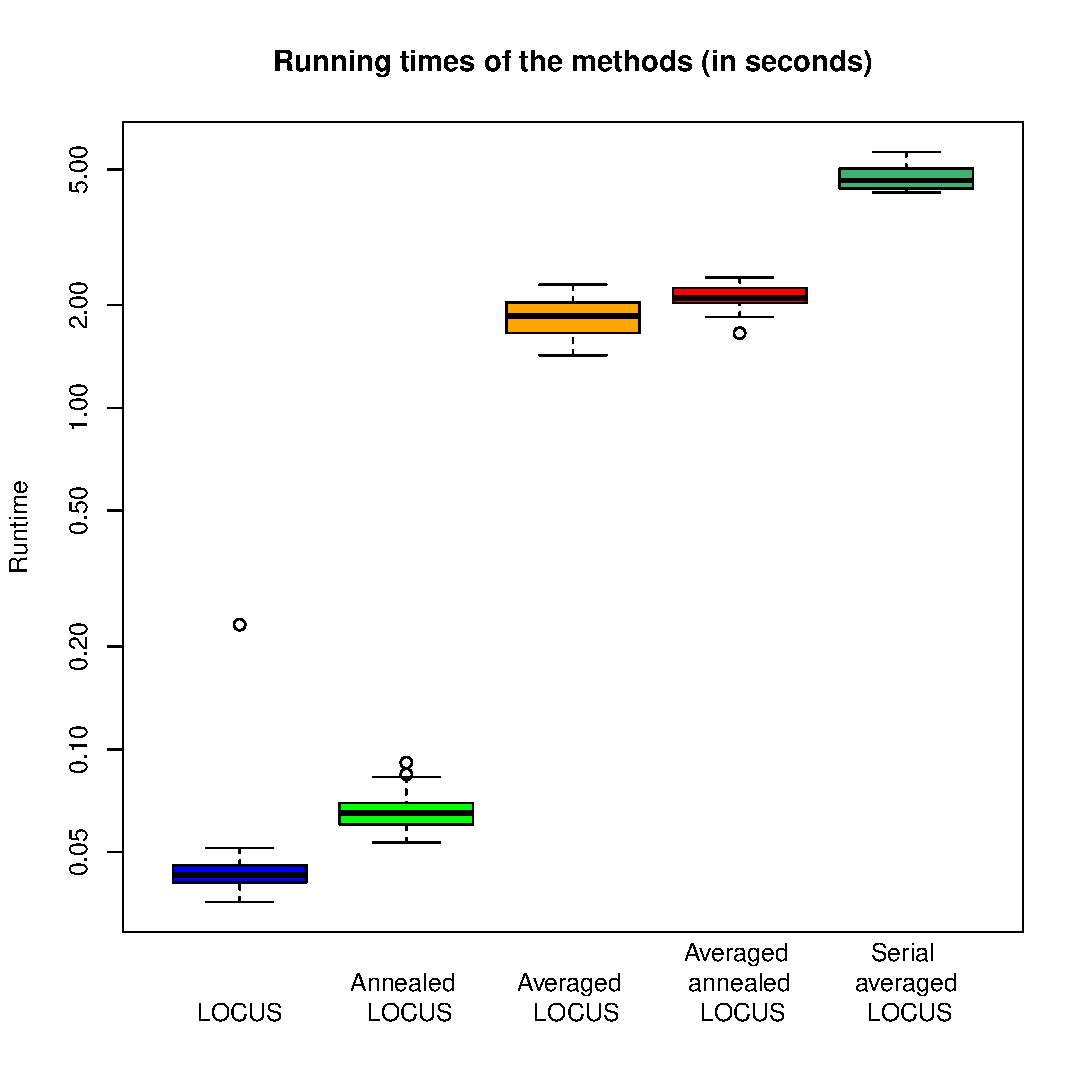
\includegraphics[width=5in,bb= 0 0 7.24in 7.24in]{images/runtime.pdf}

\caption{\label{fig:runtime} Running times, in seconds, of the methods: LOCUS (first), annealed LOCUS (second), averaged LOCUS (third), averaged annealed LOCUS (fourth), and $100$ iterations of LOCUS (fifth), computed on $300$ observations of $500$ SNPs. $15$ SNPs are associated with a single trait, and for the averaged versions, $100$ different initialisations, averaged over $50$ replications. The SNPs are correlated in blocks of ten with autocorrelation between $0.98$ and $0.99$. Up to $50\%$ of the response variance is explained by the SNPs. The times have been measured with an Intel Core i5, the methods computed in parallel used $4$ cores. The \textit{y}-axis has a logarithmic scale.}
\end{figure}

Figure \ref{fig:runtime} shows the running times of the methods, computed on $300$ observations of $500$ SNPs, $15$ SNPs associated with a single trait, and for the averaged versions, $100$ different initialisations, measured for $50$ replications. For comparison, the runtime of calculating $100$ times the LOCUS method before performing a weighted average is shown on the same figure (Serial LOCUS). The advantage of parallel implementation is highlighted, as it takes more than twice as much time to compute $100$ iterations of the LOCUS method, one after another, than to compute the averaged LOCUS method with four cores.

The averaged annealed LOCUS takes the longest to compute of the first four methods, as in addition to averaging, the method starts every occurrence with an annealing step. The annealed LOCUS also takes more time to compute than the standard LOCUS method, which confirms the additional time needed for the averaged annealing LOCUS to complete, compared to the averaged LOCUS.

The variability in the runtime of averaged annealed LOCUS is smaller than the variability in the runtime of averaged LOCUS. The annealing step of averaged annealed LOCUS yields the parameters of the different initialisations closer together, as they tend to go in the direction of the global maxima. After the annealing step, the usual algorithm takes a similar amount of time to compute for all the initialisations as the parameters it starts with are closer one from another than they were before the annealing step.
%
%
%
% ===========================================================================================================================
%
%
%
\newpage
\chapter{Conclusion}
In this work, we proposed a variational approach based on Bayesian averaging to efficiently deal with strong data correlation in genetic association problems.

We compared the variable selection performance of five methods: the original variational implementation from the package \texttt{locus} (LOCUS), our weighted average augmented method (averaged LOCUS), their simulated annealing augmented counterparts (annealed LOCUS and averaged annealed LOCUS), and the weighted average augmented method with all weights equal.

Then, we focused on the posterior distributions of the effect sizes yielded by our four methods, compared them with MCMC inference and the simulated effect sizes. With strong correlations and weak effect sizes, our methods missed an associated SNP, but found it when we weakened the correlations and augmented its effect size.

We also compared the runtime of the original implementation (LOCUS), our weighted average augmented method (averaged LOCUS), their respective simulated annealing counterparts (annealed LOCUS and averaged annealed LOCUS), and a non parallel implemented weighted averaged method.

Our proposal, averaged LOCUS, outperforms the original LOCUS method in terms of variable selection. On strongly correlated SNPs ($0.95$ to $0.99$), the averaged LOCUS has the best performance amongst the methods studied. On weaker correlated SNPs ($0.5$ to $0.95$), averaged LOCUS, with or without equal weights, annealed LOCUS, and averaged annealed LOCUS, have a similar variable selection performance.

When the correlations between the SNPs are not extremely high, it is quicker to use annealed LOCUS than to use averaged LOCUS, and it has the same variable selection performance. However, on extremely strongly correlated data, averaged LOCUS has a better performance than annealed LOCUS and averaged annealed LOCUS, and is quicker to compute than averaged annealed LOCUS.

Several improvements may be considered. First, we also need to evaluate the method performance when considering more that one trait, i.e., $q > 1$. Real eQTL data have more than one trait, so it would be better to assess the performance of the methods on relevant data. Based on \citet{glob_loc}, annealing should be important in the assessment of active SNPs.

Second, we assumed that every model is a priori equiprobable in the averaged LOCUS procedure; other choices could be considered. For example, we could relate the model probability with the expected number of associated SNPs.

Third, for the annealing procedure, we have chosen a geometric schedule, a number of steps $L$, and an initial temperature $T_L$. It would be good to compare the performance with different choices of initial temperatures, steps, and schedule.

Fourth, we would like to apply this method on real eQTL data.

Finally, provided that all our experiences show good performance, we will optimise our code and integrate it in the \texttt{locus} package (http://github.com/hruffieux/locus).
\newpage
\bibliography{references}
\bibliographystyle{apalike}
\end{document}